% This file: 			Draft Compiling New Information and Analysis
% Contributors: 		Pietro Biroli, Daniela Del Boca, Linor Kiknadze,
%					Yu Kyung Koh, Sylvi Kuperman, Sidharth Moktan,
%					Chiara Pronzato, Anna Ziff
% Original date: 		10/3/16
% Project: 			Reggio Evaluation

\documentclass[12pt]{article}
\usepackage[top=1in, bottom=1in, left=1in, right=1in]{geometry}
\parindent 22pt

\usepackage{adjustbox}
\usepackage{amsmath}
\usepackage{amssymb}
\usepackage{array}
\usepackage{booktabs}
\usepackage{datetime}
\usepackage{fancyhdr}
\usepackage{float}
\usepackage{graphicx}
\usepackage[colorlinks=true,linkcolor=blue,urlcolor=blue,anchorcolor=blue,citecolor=blue]{hyperref}
\usepackage{lscape}
\usepackage{multirow}
\usepackage{natbib}
\usepackage{setspace}
\usepackage{tabularx}
\usepackage[colorinlistoftodos,linecolor=black]{todonotes}
\usepackage{appendix}
\usepackage{pgffor}
\usepackage{caption} 
\usepackage{threeparttable}
\captionsetup[table]{skip=3pt}

\settimeformat{hhmmsstime}

\newcolumntype{L}[1]{>{\raggedright\arraybackslash}p{#1}}
\newcolumntype{C}[1]{>{\centering\arraybackslash}p{#1}}
\newcolumntype{R}[1]{>{\raggedleft\arraybackslash}p{#1}}


\externaldocument{reggioEvaluation_appendix}

\begin{document}

\title{\Large \textbf{Evaluation of the Reggio Approach} \\ Draft}
\author{\normalsize Reggio Team}
\date{\normalsize Original version: October 3, 2016 \\ Current version: \today}
\maketitle

\textbf{[JJH: Many questions -- we are not apologists for Reggio. The \emph{ad hoc} adjustment to matching bothers me. I do not see a good justification and $\Pi$ is estimated. Let's finish. We need to: (1) Put the infant toddler outcomes in main text. We have results. The fact that they are not present in other cities is a huge advantage. (2) Report step down for each column and each table. (3) Identify in each table the group being studied. (4) In the text, we need to summarize main finding of appendix in the text.]}

\tableofcontents

\clearpage
\doublespacing

\section{Introduction}
\label{sec:introduction}
Evidence from seminal experiments in early childhood interventions, such as the Perry Preschool Program, demonstrates the potential for early childhood education to improve life-cycle outcomes of disadvantaged individuals \citep{Heckman_Moon_etal_2010_QE, Elango_Hojman_etal_2016_Early-Edu}. There are many early childhood interventions that are widely replicated with little empirical evidence of their effectiveness. One such intervention is the Reggio Approach (RA). Starting in 1963 in Reggio Emilia in Northern Italy, the RA is still implemented in the municipal schools of Reggio Emilia, as well as replicated internationally.\footnote{The official \href{http://www.reggiochildren.it/network/?lang=en}{Reggio Children International Network} is present in 33 countries worldwide. Many other preschools around the world are ``inspired'' by the Reggio Approach but they are not officially part of these network.}

This paper presents an evaluation of the Reggio Approach early childhood education system in Reggio Emilia, which includes infant-toddler centers (ages 0-3) and preschools (ages 3-6). The Reggio Approach is administrated through the municipal government of Reggio Emilia. Other early childhood education options include state preschools and private infant-toddler centers and preschools. We have collected data on individuals who have attended all these types of early childhood education as well as those who were informally taken care of outside of a center setting. 

Our sample includes individuals across five age cohorts: three cohorts of adults, one cohort of adolescents, and one cohort of children in their first year of elementary school. The individuals are not only from Reggio Emilia, but also from Padova and Parma, two cities that are similar to Reggio Emilia along several dimensions but have different preschool systems. 

Evaluating the Reggio Approach presents several challenges, given the non-experimental nature of the program. The Reggio Approach preschool system was introduced in 1963, grew over the decades, and now has infrastructure to teach educators about the Reggio Approach. Therefore, he evaluation strategy has to account for potential changes in treatment over time, lack of well defined control group, and potential spillover of the Reggio Approach into other programs attended by individuals in the data. 

This analysis \ldots We find \ldots

In Section~\ref{sec:eceexperiences}, we describe the Reggio Approach and the other early childhood education experiences in the three cities focusing on administrative changes that might have led to a diffusion of aspects of the Reggio Approach. We also present an overview of the demographic aspects of Reggio Emilia, Parma, and Padova that contextualize the differences in approaches to early childhood education. Section~\ref{sec:data} describes the data in more detail and discusses the outcome variables that are available for the different cohorts. Section~\ref{sec:methodology} discusses the methodology we employ to produce the results discussed in Section~\ref{sec:results}. Section~\ref{sec:conclusion} concludes.


\section{Early Childhood Programs in Northern Italy}
\label{sec:ece-italy}
We first list the different types of early childhood education in Italy. We then describe the Reggio Approach, which we consider to be the treatment in this evaluation. Because those who did not receive this treatment did not receive a homogenous alternative early childhood education experiences, we also document the curricular and programmatic elements of these alternative programs.

\subsection{Types of Early Childhood Education in Italy}

In Italy, the responsibilities for the funding and provision of early childhood care and education are as follows: the state passes laws, defines educational aims, and provides the majority of funding for schools to regions through the Health Ministry. Each region may pass laws regarding the organization and basic planning of centers in that region. Municipalities organize and run the schools \citep{Becchi-Ferrari_1990_Pub-Inf-Centres-Italy}. 

Municipalities are further enabled to set eligibility criteria for public early childhood education. Selection criteria are similar across municipalities, however, the weighting of distinct family characteristics varies \citep{Del-Boca-etal_2016_CESifo-ES}. State preschools are free to all families with fees for meals and transportation. Fees to attend municipal schools vary; about half of municipalities provide free early childcare while others are offered on a sliding scale.

The Catholic Church offers the majority of private religious early childhood programs. Tuition is the family's responsibility, depending on income and amount of state subsidy available as decided by the municipality. Private secular early childhood programs tend to be the sole responsibility of the family \citep{Hohnerlein_2009_Paradox-Public-Preschools}.

To summarize, early childhood education is publicly provided by the municipality or the state, and privately provided by religious institutions or secular ones. \\

\noindent \textbf{[AZ: The rest of this section is outlined below. We will fill in as we receive more information from the surveys.]}

\begin{enumerate}
	\item Reggio Approach
		\begin{enumerate}
			\item Pedological influences
			\item Historical context of emergence of Reggio Approach
			\item Description of key components and approaches
		\end{enumerate}
	\item Other schools in Reggio Emilia
		\begin{enumerate}
			\item Discuss influence of Malaguzzi
		\end{enumerate}
	\item Schools in Parma and Padova 
		\begin{enumerate}
			\item Use information from surveys
		\end{enumerate}	
\end{enumerate}

%The Reggio Approach is a form of progressive early childhood education designed by Loris Malaguzzi, an educator influenced by the educational practices and psychological theories of Ciari, Dewey, Piaget, Erikson, Vygotsky, Bronfenbrenner, Kagan, and Gardner. \textbf{[AZ: Perhaps we should briefly describe some of the theories and cite these individuals instead of listing the individuals?} The Reggio Approach emerged from political conflict between the secular and communist left and the religious and conservative right. Malaguzzi was one of several left-wing educators within the region of Emilia Romagna. Under the guidance of Malaguzzi, Reggio Emilia opened its first preschool in 1963 for children aged 3-6 years. In 1965 \textbf{[AZ: Should this be 1971?]}, Reggio Emilia opened the first infant-toddler center for children aged 3 months to 3 years. The Reggio Emilia municipal system with this progressive model preceded reforms in the 60s and 70s that established state-run infant-toddler centers and preschools.
%
%In the Reggio Approach, preschool-aged children are active learners, or ``researchers." Curriculum is viewed as an ongoing, collaborative project, in contrast to a pre-defined set of learning activities. Children's developing knowledge is expressed in creative forms and documented in portfolios that are subsequently shared with the parents and children. 
%
%The Reggio Approach infant-toddler center opens at 8am. Families can choose three options for pick-up: 1 p.m. (part-day), 4 p.m. (full-time), and until 6:20 p.m. (extended day). Teachers in the infant-toddler center generally have lower initial training and receive less pay. The atelierista is not part of the infant-toddler center, but in Reggio Emilia, teachers are trained by atelieristas from the preschools. In contrast to the Reggio Approach preschool, teachers are assigned to children in single-year increments \citep{Cagliari-etal-eds_2016_BOOK_Loris-Malaguzzi,Giudici-Nicolosi_2014_Reggio-Approach}.
%
%Preschools are open five full-time days per week from September through July \citep{Giudici-Nicolosi_2014_Reggio-Approach}. The educative team is assigned specialized roles. Each class is led by two full-time co-teachers, and each school site has one full-time atelierista, an instructor with a background in visual arts. Auxiliary site staff, such as cooks and janitors, are considered members of the educative staff and are included in all trainings. A pedagogista, with a higher degree in psychology or education, is assigned to support professional development for the educative staff of approximately 4-5 schools. In addition to having an atelierista, each school is equipped with an in-house kitchen and is has an open interior design.  
%
%Teachers remain with the same group of children for three consecutive years, and thus have extended time to know each child and their families. There is no predetermined curriculum enacted by educators in that there are no distinct timelines or institutionally-prescribed content knowledge that educators must convey to achieve ``school readiness." In contrast, educators, children (and sometimes families) collaborate to define a question or topic and pursue research that is not constrained by a predetermined timeline. Teachers observe, scaffold learning, and engage children in discussion. Children demonstrate their emerging knowledge through creative visual media, aided by the atelierista. Teachers document each child's development in a portfolio---a collection of work---which is reviewed and discussed with children and parents over the year. 
%
%\subsection{Other Early Childhood Education Experiences}
%
%Municipal early childhood education programs in Reggio Emilia, Parma and Padova differ in certain aspects of program administration, environmental features, and pedagogical methods. We discuss these differences below. 
%
%\subsubsection{Parma}
%
%Published literature documenting the Parma municipal early childhood system in detail is scarce. Carolyn Pope Edwards suggests that municipal schools in Parma are parallel to those of Reggio Emilia.\footnote{Kuperman, Interview with Carolyn Pope Edwards, 2016. See \citet{Edwards-etal-eds_1998_Hundred-Languages}.} 
%
%As of 2001, 16 infant-toddler centers were offered throughout the municipality. The administration of these centers are managed by a director of services for children under 3 years of age. Pedagogical coordinators perform both administrative and professional development roles. Assigned to a specific set of infant-toddler centers, they meet twice each month with all site teachers collectively for shared reflection, on-site supervision, and to promote relationships with families. The city director meets biweekly with all pedagogical coordinators for overall planning. University professors or administrators from other municipalities provide professional development in the form of continuing education \citep{Terzi-Cantarelli_2001_Parma}.
%
%In contrast to pre-fabricated preschool centers, Parma's infant-toddler centers are intentionally designed in the context of an apartment. \citet{Terzi-Cantarelli_2001_Parma} report mixed-age classes that include 18 total children from 13 months to 3 years in a single section, led by two teachers (9:1 child-teacher ratio). To accommodate parents, infant-toddler centers open at 7:30pm and offer 3 pick-up times: 2 p.m. (short-day), 3:30 p.m. (normal-day), or 5 p.m. (extended-day). Classrooms can be organized by single-age groups (e.g., 5-12 months, 12-24 months, and 24-36 months) or by mixed-age groups (e.g.,12-36 months) \citep{Majorano-etal_2009_CC-in-P}.
%
%\textbf{[AZ: Information on preschool in Parma]}
%
%\subsubsection{Padova}
%Padova is located in the relatively more religious and politically diverse region of Veneto. Compared to Reggio Emilia and Parma, its municipal early childhood education system is smaller and it has a higher number of private religious programs. 
%
%In 1989, the region of Veneto reported a total provision of childcare slots for 3.9\% of its infant-toddler population. In contrast, the region of Emilia Romagna reported a provision of infant-toddler childcare for 15.6\% of its population. The practice of professional development trainings for early childhood staff in Veneto first began in 1986. \textbf{[AZ: citation?]}
%
%The Catholic Church offers the majority of private religious early childhood programs; tuition is the family's responsibility, depending on income and amount of state subsidy available as decided by the municipality \citep{Hohnerlein_2009_Paradox-Public-Preschools}.  A major concern of the Catholic Church in Italy is equity and parity of state funding for private schools.\footnote{In 2005, funding for state and private schools differed greatly. Authorized private schools received a state contribution for pre-primary schools (ages 2-6 years), while funding for private primary schools (ages 6-11 years) was at 15.5\% the rate of public primary schools. Private secondary schools (ages 11-18 years) received no state funding. \textbf{[AZ: citation?]}}
%
%Prior to March 2000, state funding for private schools reflected a 1947 constitutional clause that non-state schools could operate ``without financial burdens on the state.'' Private schools were thus considered options only for affluent families that could afford the tuition expense. \textbf{[AZ: citation?]}


\section{Research Design}
\label{sec:data}
\subsection{The Selection of Cities}

Our dataset contains cohorts of individuals raised in Parma and Padova, in addition to Reggio Emilia. Parma and Padova are similar to Reggio Emilia in terms of geography, population, and socio-economic structure, but they do not have the Reggio Approach available.\footnote{Other Italian cities were taken into consideration, notably Brescia, Livorno, Modena, Perugia, Piacenza, Prato, and Ravenna. Parma and Padova were the two cities that best fulfilled our comparability and sample requirements.} 

All three cities are in Northern Italy with Parma and Reggio Emilia being in the same state and Padova being in the neighboring one. In addition to geographic proximity, they have similar populations as seen in Figure~\ref{fig:population}. Although the population in Padova is higher than in Parma and Reggio Emilia, the trends are similar across time. These similar trends can also be seen in the migration rates between the three cities (Figure~\ref{fig:emigr-immigr}). Although emigration rate is highest in Padova and net migration rate is highest in Reggio for most of the years, general trends in emigration and immigration in similar in all cities. Trends in foreign migration are almost identical in three cities. 

The similarities between the cities are also seen in economic terms. Reggio Emilia has an average per-capita income of 25,226 euros, Parma of 28,437, and Padova of 29,915 in 2011 \citep{Comuni-Italiani_2017_Redditi-Ipref-per-Regione-2011}. Other economic information, such as unemployment, is similar across the cities as well. We present more information on the three cities in Appendix~\ref{sec:data-app}.

\begin{figure}[H]
      \centering
        \begin{subfigure}[t]{0.49\textwidth}
          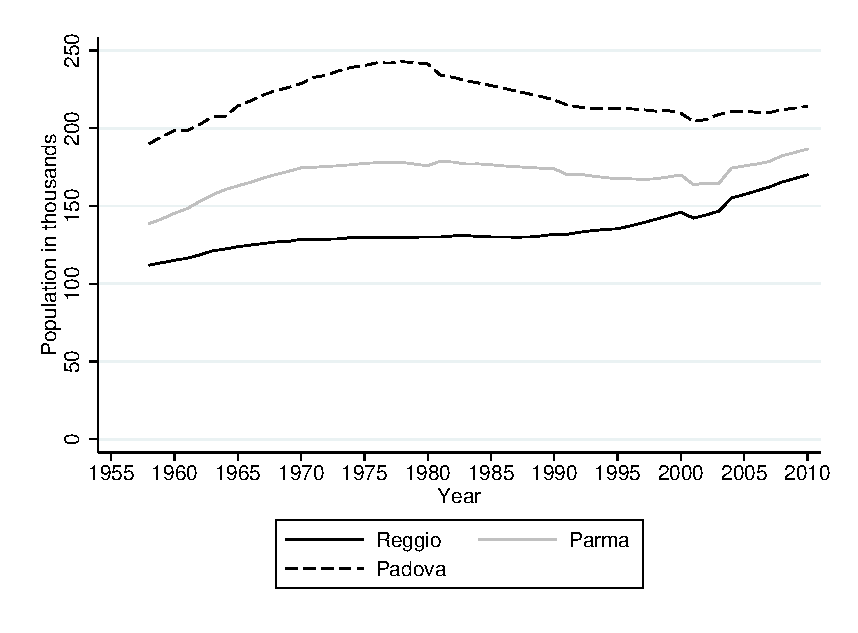
\includegraphics[width=\textwidth]{../../output/image/population.eps}
\caption{Population}
        \end{subfigure}
        \begin{subfigure}[t]{0.49\textwidth}
          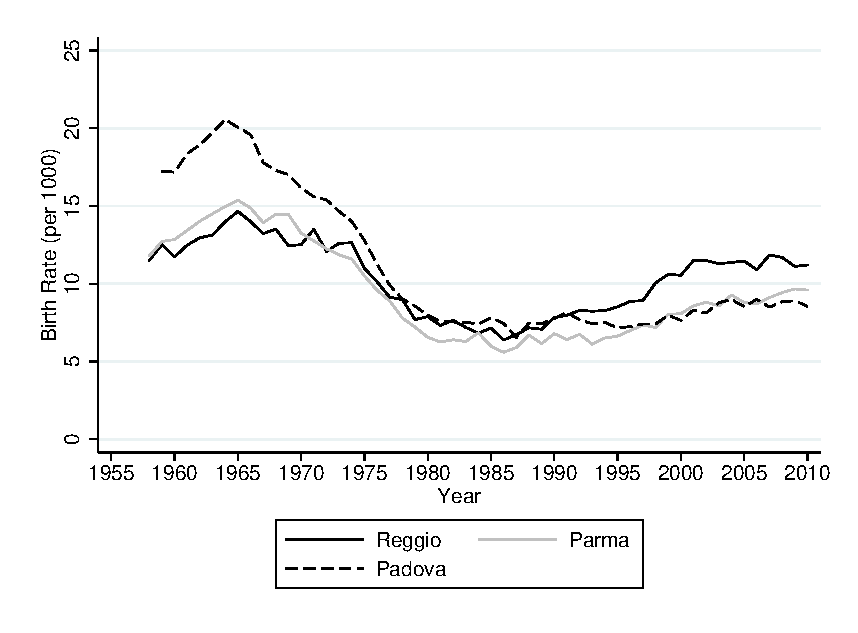
\includegraphics[width=\textwidth]{../../output/image/birth_rate.eps}
 \caption{Birth Rate}
        \end{subfigure}
        \begin{subfigure}[t]{0.49\textwidth}
          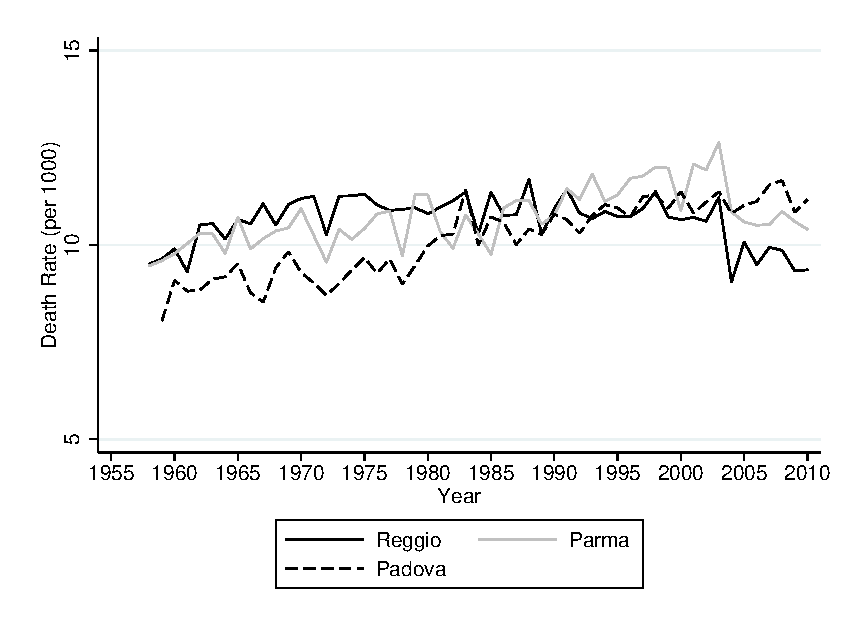
\includegraphics[width=\textwidth]{../../output/image/death_rate.eps}
        \caption{Death Rate}
        \end{subfigure}
        \begin{subfigure}[t]{0.49\textwidth}
          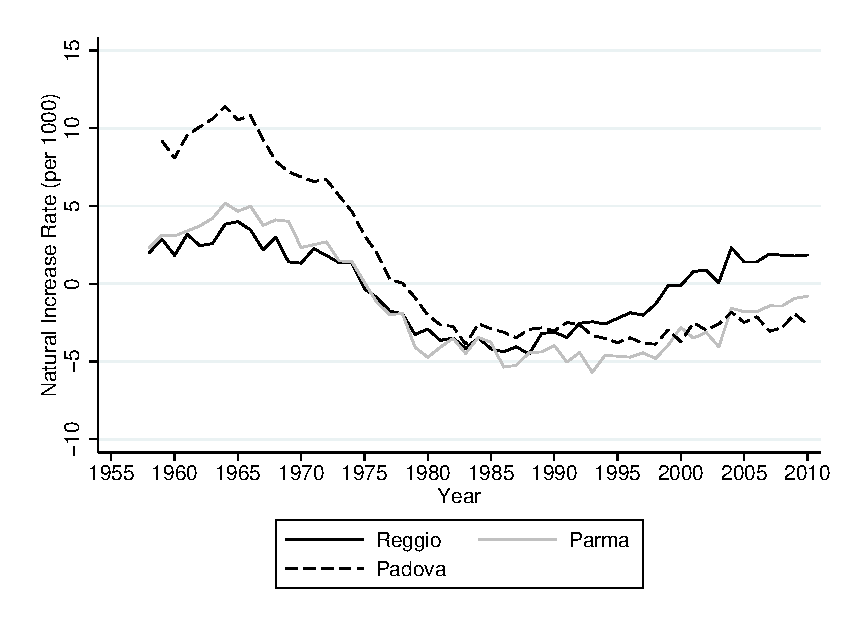
\includegraphics[width=\textwidth]{../../output/image/naturalinc_rate.eps}
            \caption{Natural Rate}
        \end{subfigure}
      \caption{Population Statistics}  \label{fig:population}
    \end{figure}

\textbf{[JJH: Can we test for equality across cities?]}

\begin{figure}[H]
      \centering
        \begin{subfigure}[t]{0.49\textwidth}
          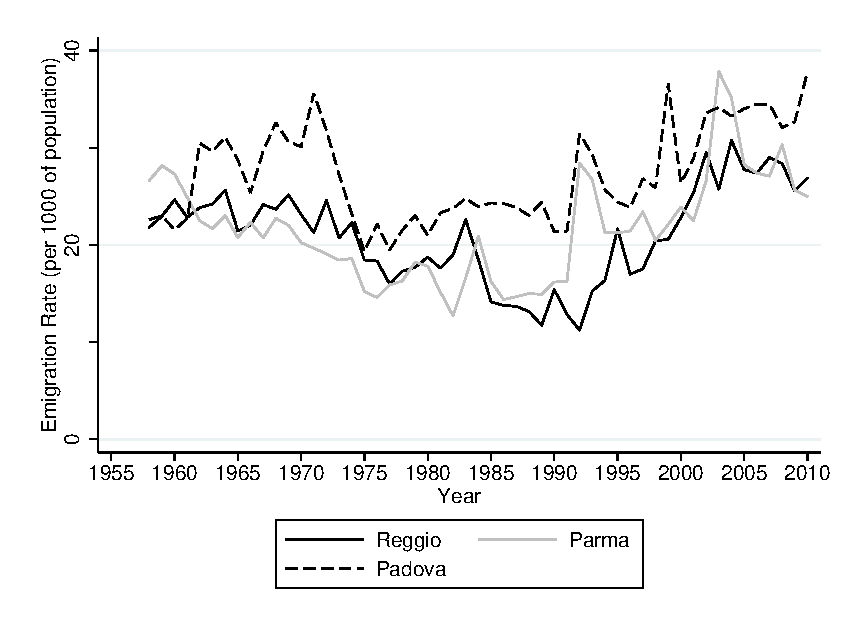
\includegraphics[width=\textwidth]{../../output/image/emigration.eps}
            \caption{Emigration}
        \end{subfigure}
      \begin{subfigure}[t]{0.49\textwidth}
        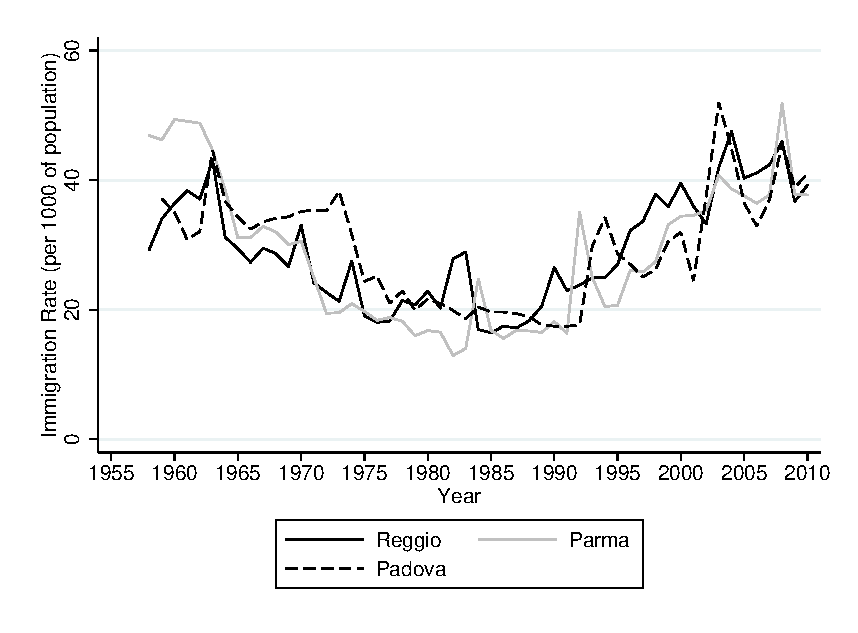
\includegraphics[width=\textwidth]{../../output/image/immigration.eps}
        \caption{Immigration}
      \end{subfigure}
	 \begin{subfigure}[t]{0.49\textwidth}
          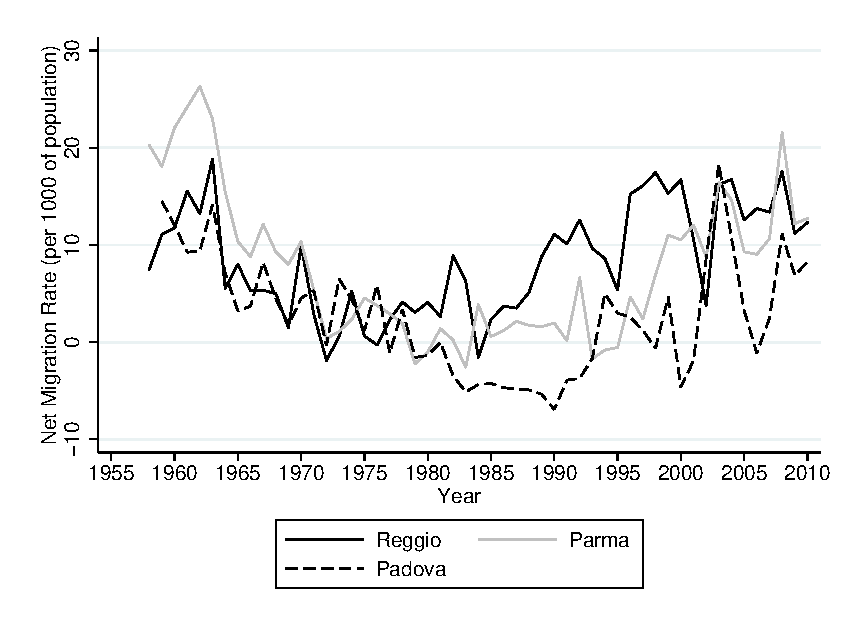
\includegraphics[width=\textwidth]{../../output/image/netmigration.eps}
\caption{Net Migration}
        \end{subfigure}
        \begin{subfigure}[t]{0.49\textwidth}
          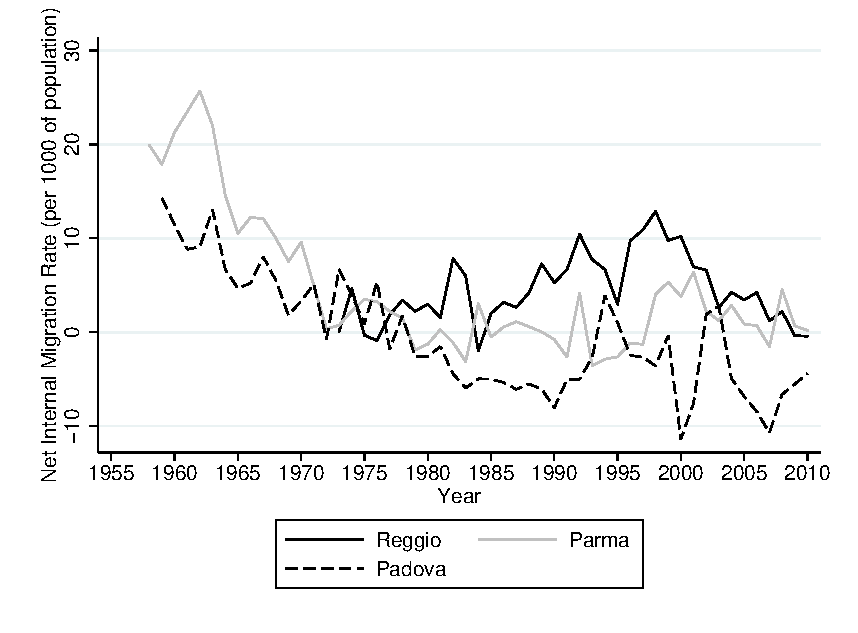
\includegraphics[width=\textwidth]{../../output/image/netinternalmig.eps}
 \caption{Net Internal Migration}
        \end{subfigure}
        \begin{subfigure}[ht]{0.48\textwidth}
          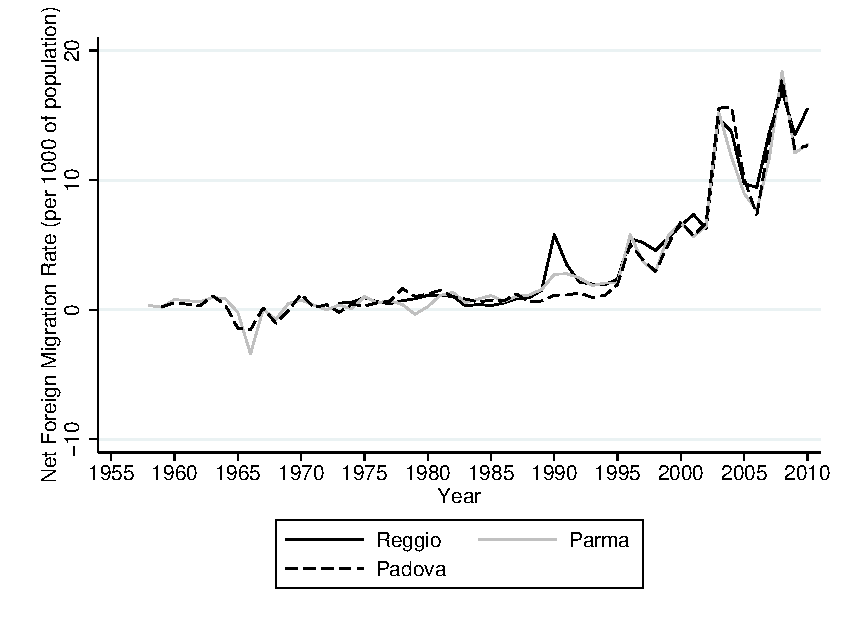
\includegraphics[width=\textwidth]{../../output/image/netforeignmig.eps}
        \caption{Net Foreign Migration}
        \end{subfigure}

      \caption{Migration Statistics}  \label{fig:emigr-immigr}
    \end{figure}
\subsection{The Selection of Cities}
Section \ref{sec:eceexperiences} shows that the childcare systems within and outside Reggio Emilia share the Reggio Approach components to varying degrees. Because other childcare options may be similar to the Reggio Approach to some extent and may have their own high-quality components, it is difficult to evaluate the clean effects of the Reggio Approach. Our survey data collection is designed to evaluate the impact of the Reggio Approach relative to other programs that share similar components. Note that our comparison is not to determine whether Reggio is of higher or lower quality relative to other programs but to understand how the programs are different across school types, cities, and over time. 

We collect data on the individuals in Reggio Emilia, Parma, and Padova. Parma and Padova
have been chosen in addition to Reggio Emilia to represent appropriate controls: they are close enough to
Reggio Emilia in terms of size, geographic, demographic, and socio-economic
structure, but they did not experience its unique approach to early
childhood education.\footnote{%
Other Italian cities were taken into consideration, notably Brescia,
Livorno, Modena, Perugia, Piacenza, Prato, and Ravenna. Parma and Padova
were the two cities that best fulfilled our comparability and sample
requirements.} For example, Reggio Emilia has a population of roughly
173,000, Parma of 188,000, and Padova of 210,000 in 2013.\footnote{%
The population size in December 2013 was 172,525 in Reggio Emilia, 187,938
in Parma, and 209,678 in Padova. Source: ISTAT, %
\url{http://www.demo.istat.it/}} Also their economic resources are
comparable: Reggio Emilia has an average per-capita income of 25,226 euros,
Parma of 28,437, and Padova of 29,915 in 2011.\footnote{%
Source: Finance Minister, taxable income for 2011.} 
%See \url{http://www.comuni-italiani.it/statistiche/redditir2011.html}
Even more importantly, these three cities face analogous fertility dynamics
and, consequently, potential demand for child-care services. The three
cities had a very similar number of births from both Italians and immigrants
in the past decade. Parma is a neighboring city 30 km to the west of Reggio
Emilia, it belongs to the same administrative region of Emilia-Romagna, and
shares with Reggio a common background that forged the city's political and
economic system, and shaped its culture and social capital; yet Parma has
witnessed a different approach to public investment in early childhood
education. On the contrary, Padova lies 150 km away from Reggio Emilia, in
the richer north-eastern region of Veneto, and was more influenced by the
history and culture of Venice. Yet, Padova, just as Reggio Emilia, is a middle-size
Italian city with a thriving migrant population, facing similar political
and economic issues, with a different social background but similar
resources which can be devoted to early childhood education.

Figure \ref{fig:enrollment} explores the similarities and difference in enrollment statistics in three cities. Note that enrollment data is not available for Parma except for the year 2010. It is shown that Padova has the highest rate of attending preschool. It is also shown that Reggio Emilia and Padova observed the increase in preschool enrollment; from the 1990s, almost all children of age 3-5 are enrolled in preschool. The figures also show that the percentage of enrollment in municipal preschools increased during the 1970s and the 1980s in Reggio Emilia and Padova, but decreased after the 1990s in Reggio Emilia. The percentage enrolled in state preschools increased over time in both Reggio Emilia and Padova. In contrast, the percentage enrolled in private preschools decreased over time in Reggio Emilia and Padova. For Parma, the enrollment statistics in 2010 are similar to those of Reggio Emilia. 
 
\begin{figure}[H]
      \centering
        \begin{subfigure}[t]{0.49\textwidth}
          \includegraphics[width=\textwidth]{../../output/image/enroll_num_graph.eps}       
\caption{Num. of Children Enrolled in Preschool}        
        \end{subfigure}
        \begin{subfigure}[t]{0.49\textwidth}
          \includegraphics[width=\textwidth]{../../output/image/enroll_per_graph.eps}       
 \caption{Percentage of Ages 3-5 Enrolled in Preschool}        
        \end{subfigure}
        \begin{subfigure}[t]{0.49\textwidth}
          \includegraphics[width=\textwidth]{../../output/image/enroll_per_muni_graph.eps} 
        \caption{Percentage of Enrollment in Municipal Preschool}        
        \end{subfigure}
        \begin{subfigure}[t]{0.49\textwidth}
          \includegraphics[width=\textwidth]{../../output/image/enroll_per_stat_graph.eps}
            \caption{Percentage of Enrollment in State Preschool}       
        \end{subfigure}
      \begin{subfigure}[ht]{0.48\textwidth}
        \includegraphics[width=\textwidth]{../../output/image/enroll_per_priv_graph.eps}
        \caption{Percentage of Enrollment in Private Preschool}
        \label{fig:large}
      \end{subfigure}
      \caption{Enrollment Statistics}  \label{fig:enrollment}
    \end{figure}


\subsection{The Survey Data Collection}

The individuals were collected from the population registries in each of the cities in the year ranges of the five cohorts. The sample was then restricted to those individuals living in the same city in which they were raised. All cohorts. except the youngest one, are restricted to individuals who are Italian citizens. In contrast, the youngest cohort includes an oversampling of immigrant children.\footnote{In the adult cohorts there was no immigrant who was preschool age in the same school in which they live. In the adolescent cohort, the number was immigrant born was extremely small.} The sample from Reggio Emilia, across all cohorts, includes an oversampling of those who attended municipal schools, as this is considered the treatment group.

Of the reference sample, 7,109 individuals were randomly selected. Of these, 4,019 completed interviews, resulting in a response rate of 56.5\%. Table~\ref{tab:sample-city-cohort} provides an overview of the birth years for the different cohorts and the counts of the full sample.
\begin{table}[H]
\centering
\begin{threeparttable}
	\caption{Description of the Full Sample by Cohort and City}\label{tab:sample-city-cohort}
	\begin{tabular}{l c c c c c c}
\toprule
Cohort & Birth year(s) & Age at interview & \mc{4}{c}{Count} \\
\cmidrule{4-7}
 & 		&						& Reggio Emilia & Parma & Padova & \textbf{Total} \\
\midrule
Children & 2006 & 6 & 311 & 291& 278 & 880 \\
Migrants & 2006 & 6 & 110 & 58 & 113 & 281 \\
Adolescents & 1994 & 19 & 300 & 254 & 282 & 836 \\
Adults 30s & 1980-1981 & 32 & 280 & 251 & 251 & 782 \\
Adults 40s & 1969-1970 & 43 & 285 & 254 & 252 & 791 \\
Adults 50s & 1954-1959 & 54-60 & 200 & 103 & 146 & 449 \\
\midrule
\textbf{Total}	& 				& & 1,486 & 1,211 & 1,322 & 4,019 \\
\bottomrule
\end{tabular}
\begin{tablenotes}
\footnotesize
Note: This table presents the number of individuals in the full sample. The age at interview is an approximation given there is some variation in the interview date and birth year within each cohort. In analysis, we combine the Italian and migrant subsamples of the child cohort and control for migrant status.
\end{tablenotes}
\end{threeparttable}
\end{table}

Table~\ref{tab:sample} provides a detailed tabulation of the sample by city, cohort, and school type. It shows that the number of people who do not attend any preschool decreases over time. Whereas the majority of individuals from the age-50 cohort did not attend any preschool, there are few such cases in the child and adolescent cohorts. Table \ref{tab:sample} also shows that the proportion of individual attending municipal preschools is higher in Reggio Emilia than in the other cities.\footnote{This is due to the construction of the sample.} Note that the Reggio Approach preschools were not available for the age-50 cohort, as demonstrated in Table \ref{tab:itc-pre} and Table \ref{tab:sample}. 

\begin{table}[H]
\centering
\scalebox{0.85}{
\begin{threeparttable}
	\caption{Tabulation of Preschool Attendence by Cohort, City, and School Type}\label{tab:sample}
	\begin{tabular}{l*{8}{c}}
\toprule
	&	\mc{7}{c}{Reggio Emilia: 1,486}													\\	\midrule
	&	None	&	Muni	&	State	&	Reli	&	Priv	&	Muni-Affi	&	Other	\\	\midrule
Children	&	2	&	159	&	44	&	92	&	5	&	7	&	1	\\	
Migrants	&	4	&	47	&	38	&	14	&	1	&	3	&	1	\\	
Adolescents	&	7	&	151	&	22	&	98	&	6	&	13	&	0	\\	
Adults 30s	&	57	&	138	&	31	&	40	&	1	&	4	&	8	\\	
Adults 40s	&	80	&	87	&	14	&	52	&	5	&	1	&	43	\\	
Adults 50s	&	147	&	0	&	0	&	29	&	2	&	0	&	20	\\	\midrule
	&	\mc{7}{c}{ Parma: 1,211}													\\	\midrule
	&	None	&	Muni	&	State	&	Reli	&	Priv	&	Muni-Affi	&	Other	\\	\midrule
Children	&	5	&	105	&	42	&	74	&	8	&	52	&	0	\\	
Migrants	&	4	&	25	&	12	&	3	&	6	&	7	&	0	\\	
Adolescents	&	4	&	100	&	52	&	77	&	6	&	5	&	2	\\	
Adults 30s	&	44	&	85	&	56	&	51	&	5	&	4	&	3	\\	
Adults 40s	&	116	&	0	&	0	&	55	&	1	&	4	&	73	\\	
Adults 50s	&	72	&	0	&	0	&	11	&	0	&	10	&	9	\\	\midrule
	&	\mc{7}{c}{Padova: 1,322}													\\	\midrule
	&	None	&	Muni	&	State	&	Reli	&	Priv	&	Muni-Affi	&	Other	\\	\midrule
Children	&	2	&	58	&	45	&	141	&	12	&	19	&	0	\\	
Migrants	&	5	&	33	&	46	&	23	&	1	&	0	&	4	\\	
Adolescents	&	1	&	84	&	46	&	132	&	6	&	7	&	2	\\	
Adults 30s	&	47	&	27	&	27	&	140	&	1	&	7	&	0	\\	
Adults 40s	&	75	&	0	&	0	&	126	&	0	&	10	&	39	\\	
Adults 50s	&	57	&	0	&	0	&	72	&	2	&	6	&	3	\\	

\bottomrule
\end{tabular}


\begin{tablenotes}
Note: This table shows the sample size by city, cohort, and school type. We separate migrants and children for clarity in this table even though they are in the same birth cohort (year of birth: 2006). None: no preschool; Muni.: municipal preschool;  State: state preschool; Relig.: religious preschool; Priv.: private preschool. Muni-Affi: municipal-affiliated preschool; Other: uncategorized preschool.
\end{tablenotes}
\end{threeparttable}
}
\end{table}

The structure of the cohorts allows us to study the effects of the Reggio Approach at different points throughout the life cycle. The children in the youngest cohort were interviewed when they entered primary school, the adolescent cohort when they ended compulsory schooling, and the adult cohorts capture different points of adulthood to measure key outcomes such as engagement in the labor market, health, and family decisions. This cohort structure also allows us to evaluate the Reggio Approach compared to the alternative early childhood experiences over time.

Restricting the sample to individuals living in the same city in which they were raised is necessary because of the municipal structure of the population registries. If the Reggio Approach has a treatment effect on migration out of Reggio Emilia, then our sample might oversample individuals with characteristics that are not predictive of emigration. Table~\ref{tab:immigration} presents the proportion of people who were born in Italy, of Italian citizenship, and then still resident in that town of birth, out of the total number of names given by the population registries. For all cohorts, the immigration rates are very similar for all three cities. This reinforces our choice of treatment and control cities, which share a similar economic and labor market history. Nonetheless, it is worth noting that embedded in our sample selection is the potential bias due to the fact that one of the effects of preschool might be a higher propensity to emigrate. 

\begin{table}[H]
\centering
\begin{threeparttable}
	\caption{Percentage of People Living in the Same City Since Birth}\label{tab:immigration}
	\begin{tabular}{ l c c c c }
\toprule
\textbf{Cohort} & \textbf{Reggio (\%)} & \textbf{Parma (\%)} & \textbf{Padova (\%)} & \textbf{Total (\%)}\\
\midrule
Italian Children born in 2006 (Cohort V)   & 61.3  & 70.2  & 65.1  & 65.2 \\[0.2em]
Adolescents born in 1994 (Cohort IV)       & 58.1  & 63.0  & 64.4  & 61.9 \\[0.2em]
Adults born in 1980-81 (Cohort III)        & 26.5  & 27.5  & 32.6  & 29.0 \\[0.2em]
Adults born in 1969-70 (Cohort II)         & 27.9  & 31.6  & 31.9  & 30.6 \\[0.2em]
Adults born in 1954-59 (Cohort I)          & 28.8  & 27.9  & 31.4  & 29.5 \\[0.2em]
\midrule
\textit{Total}         & \textit{32.3\%}  & \textit{32.5\%}  & \textit{35.2\%} & \textit{33.5\%} \\
\bottomrule
\end{tabular}

\begin{tablenotes}
\footnotesize
Note: This table presents the percentage of people living in same city since birth. This  shows the reference sample who satified the selection criteria (born in the city of residence and of Italian citizenship) as a percentage of the total number of names given by the population registries.
\end{tablenotes}
\end{threeparttable}
\end{table}

\subsection{The Questionnaire Design}

The questionnaires examine impact of the Reggio Approach on various dimensions of
outcomes. People at different stages of their life-cycle were asked about
family composition, fertility, labor force participation, income, schooling,
cognitive ability, social and emotional skills, health and healthy habits,
social capital, interpersonal ties, as well as attitudes on migrants. There are three age-specific questionnaires: one for the
Italian and immigrant child cohorts, one for the adolescent cohort, and one for the adult cohorts.

The child and adolescent questionnaires are further divided in
two main parts: one answered by the caregiver, with questions about the
child but also about herself and her family, and a second part answered
directly by the child or adolescent. Two survey modes have been tested and
piloted to achieve the optimal wording, timing, and length\footnote{By
means of a first pilot in the city of Bergamo with a sample from every
cohort, and a second pilot in Reggio Emilia, Parma, and Padova on a
subsample of adults, the questionnaires were tested and refined to the final
version, which lasts approximately 40 minutes for the adults, and 1 hour for
the children and the adolescents.}: a face-to-face
Computer Assisted Personal Interview (CAPI), and a Paper And Pencil
Interview (PAPI), both of which are included in the sample data. Both contain exactly the same questions, but the CAPI is a
survey mode intended particularly for the children and all those who agree
to a face-to-face interview, while the PAPI is a survey mode targeted to
those who prefer to take their time and answer questions on their own.

The questionnaires are divided in different sections each addressing a specific domain of the
respondent's life that could be influenced by early-life experiences. These
domains can be classified into three broad categories: (1) demographic and
socio-economic characteristics of the respondents; (2) mental, social, and
emotional wellbeing; (3) attitudes toward themselves and society. In the
following we describe each of them in turn.

\subsubsection{Demographic and Socio-Economic Characteristics}

The first part of the questionnaire gathers information on the demographic
and socio-economic characteristics of the respondent's family in the
following five domains: family composition, education, labor market,
marriage, and fertility. Besides containing standard background information
on the characteristics of each member of the household, this section asks
extensive information on early-childhood education and family background.
The respondents are asked about child care choices in the first six years of
life, the name and address of any infant-toddler center and preschool
attended, the age of attendance, and the reason behind these choices. For the younger cohorts, the caregivers are
also asked about their own preschool experiences, and the children and
adolescents about their attitudes towards school. Furthermore, adults and
caregivers are surveyed about their relations with parents and grandparents,
and about grandparents' involvement in child care. In the adult questionnaire, respondents are also asked about the social,
economic, and religious background of their parents. 

\subsubsection{Mental, Social, and Emotional Wellbeing}

The Reggio Approach not only focuses on
learning, but places a great emphasis on parental involvement in education
and on the formation of health, emotional and behavioral skills, social
capital, and cognitive ability. These skills are measured in the second part
of the questionnaires with a variety of existing scales and tools as follows. First, caregivers and adults answer questions about
parenting practices using the Home Observation Measurement for the
Environment (HOME) scale, in order to evaluate the family environment of the
younger cohorts, as well as to elicit the adults' attitudes to invest in
their own children. Second, adolescents, caregivers, and adults are asked
about the physical health and the healthy habits of themselves and of their
children, including self-assessed health, eating and exercising habits, as well as drinking, smoking, and other risky
behaviors. Third, the questionnaire measures various forms of
socio-emotional skills and mental health conditions. Respondents are asked
to fill in the Strength and Difficulties Questionnaire (SDQ)\footnote{SDQ is a brief behavioural screening questionnaire about 3-16 year olds. It inquires about (1) emotional symptoms, (2) conduct problems, (2) hyperactivity/inattention, (4) peer relationship problems, and (5) prosocial behavior.}, a short
version of the Rotter Locus-of-Control Scale, the 10-item Center for
Epidemiologic Studies Depression (CES-D) Scale, questions regarding
satisfaction using Self-Anchoring Ladder \citep{Cantril_1965_BOOK_Pattern-Hum-Con}, and to report
personal stress and time usage following the ISTAT-Indagine Multiscopo
questions. Using age-appropriate scales with emoticons from the Child
Outcome Rating Scale (CORS), children are asked about their happiness and
satisfaction. Fourth, in the realm of social capital, adults and adolescents
are asked questions about social networks, discrimination, friendship ties,
religiosity, and political inclination. The children's questionnaire also
contains questions regarding friendship, reciprocity, and sharing attitudes.
Finally, at the very end of each questionnaire all the respondents take a
nonverbal IQ test: a short version of the Raven
Progressive Matrices. We modify all cognitive and noncognitive measures so that the higher value means more socially positive outcome.

\subsubsection{Attitudes Towards Self and Society}

The final category of questions focuses on the respondents' attitudes
towards themselves and society, asking about four domains: their opinions
about society, their level of trust and reciprocity, their future
inclinations, and their attitudes towards immigration. Caregivers, adults,
and adolescents are asked their opinions and satisfaction with the
public services offered by the city, their thoughts on prohibition of
alcohol and drugs, and their level of trust and reciprocity towards
strangers.\footnote{%
These same questions are used in the German Socio-Economic Panel (G-SOEP) %
\url{www.diw.de/gsoep/}. The questions about trust
were also asked to the caregivers.} Adults are also asked about their
opinion on gender and family issues, while adolescents about their
sentimental life. All these questions are asked because attending a Reggio Approach school could have
shaped the way the respondents view the world around them. Adolescents and
children also share information regarding future inclinations on career plan, marriage, and success in life. Finally, another unique feature of our questionnaires is the section that elicits the respondents' attitudes toward immigration. Adolescents, adults, and caregivers answer one of two sets of questions, according to their nationality: Italians are asked about their general opinion about immigration and their contact with foreigners; immigrants are asked about their experiences of integration within the city. Furthermore, the self-completion section of the questionnaire contains more straightforward questions about racism, immigration policy, and willingness to befriend or live next door to a foreigner.


\section{Analysis}
\label{sec:methodology}
%
Because there are two stages of early childhood interventions, (i) ages 0-3 and (ii) ages 3-6, it is important to consider both when estimating treatment effects of either intervention on later outcomes. Table~\ref{tab:cases-treat} shows the possible cases of receiving early childhood intervention in our data, where 0 indicates not attending and 1 indicates attending. At this stage, we limit the type of infant-toddler centers and preschools to municipal only. 

\begin{table}[H]
\caption{Possible Cases of Treatment} \label{tab:cases-treat}
\begin{tabular}{C{1.8cm} R{0.7cm} C{2cm} C{2cm}}
  
		& & \multicolumn{2}{c}{Preschool (Ages 3-6)} \\
		& & 0 & 1 \\ \cline{3-4}            
        								 &  & \multicolumn{1}{|c|}{} & \multicolumn{1}{c|}{} \\
        							& 0 & \multicolumn{1}{|c|}{(0,0)} & \multicolumn{1}{c|}{(0,1)} \\ 
        				ITC				&  & \multicolumn{1}{|c|}{} & \multicolumn{1}{c|}{} \\ \cline{3-4}
                        (Age 0-3)  		&  & \multicolumn{1}{|c|}{} & \multicolumn{1}{c|}{} \\
        								& 1 & \multicolumn{1}{|c|}{(1,0)} & \multicolumn{1}{c|}{(1,1)} \\ 
        								&  & \multicolumn{1}{|c|}{} & \multicolumn{1}{c|}{} \\ \cline{3-4}
\end{tabular}
\begin{flushleft}
\footnotesize{Note:} We only consider municipal ITCs (infant-toddler-centers, ages 0-3) and preschools (ages 3-6). (0,0): did not attend any municipal school for both ages 0-3 and 3-6; (1,0): attended a municipal school for ages 0-3 but did \textit{not} attend for ages 3-6; (0,1): did \textit{not} attend a municipal school for ages 0-3 but did attend for ages 3-6; (1,1): attended a municipal school for both ages 0-3 and 3-6.
\end{flushleft}
\end{table}

\subsection{Estimating Effects of Infant-Toddler Centers}
There are two main methods to test the effect of attending infant-toddler centers. The first is to compare people who did not attend infant-toddler care or preschool with people who only attended municipal infant-toddler care. Using the notation in Table~\ref{tab:cases-treat}, this comparison is between (0,0) and (1,0). The second method is to compare people who only attended municipal preschool with people who attended both municipal infant-toddler centers and preschools. That is, to compare (0,1) and (1,1). The hypotheses are formally written as
\begin{eqnarray}
H_1: &  Y_{0,0} = Y_{1,0} \\ 
H_2: &  Y_{0,1} = Y_{1,1} 
\end{eqnarray}
\noindent where $Y_{i,j}$ is the outcome of the individuals who attended $i \in \{0,1\}$ infant-toddler care and $j \in \{0,1\}$ preschool.

A possible estimation strategy is to limit the sample to a specific city and a specific cohort constrained to the comparison groups needed according to the hypotheses above. To test $H_1$, we estimate the following regression equation:
\begin{eqnarray}
Y_{i}^{c,h} & = & \alpha + \beta_{0}R_i^{ITC} + \mathbf{X}_i\gamma + \varepsilon_{i}^{c,h}, \\ \nonumber
& \forall & i \in \text{ \{People in city $c$ and cohort $h$ and in group (0,0) or (1,0)\}}
\end{eqnarray}
where $R_i^{ITC}$ is the indicator for attending municipal infant-toddler center and $\mathbf{X_i}$ is the vector of baseline variables for individual $i$. Likewise, to test $H_2$:
\begin{eqnarray}
Y_{i}^{c,h} & = & \alpha + \beta_{0}R_i^{ITC} + \mathbf{X}_i\gamma + \varepsilon_{i}^{c,h}, \\ \nonumber
& \forall & i \in \text{ \{People in city $c$ and cohort $h$ and in group (0,1) or (1,1)\}.}
\end{eqnarray}

One caveat of this analysis is that it uses a limited sample size. In our data, these hypotheses cannot be tested under this strategy for many groups. Table~\ref{tab:num-group} shows the number of individuals available for each group necessary for analysis using this strategy. It is impossible to test $H_1$ in our data, because there are almost no people who attended municipal infant-toddler care without attending preschool (the group (1,0)). While it is possible to test $H_2$ for several groups, the number of observations for the group (1,1) is small for the adult cohorts. 

\begin{table}[H] \caption{Number of Individuals in Each Group} \label{tab:num-group}
\scalebox{0.77}{
\begin{tabular}{l|ccccc|ccccc|ccccc}
\toprule
			& 		\multicolumn{5}{c}{\textbf{Reggio}}		& 	\multicolumn{5}{|c|}{\textbf{Parma}}	& 			\multicolumn{5}{c}{\textbf{Padova}}				\\
			& (0,0) & (1,0) & (0,1) & (1,1) & Total & (0,0) & (1,0) & (0,1) & (1,1) & Total  & (0,0) & (1,0) & (0,1) & (1,1) & Total \\ \midrule
Child		& 2 & 0 & 46 & 117 & \textbf{311} & 5 & 1 & 35 & 100 & \textbf{291} & 2 & 0 & 31 & 36 & \textbf{278} \\
Migrant		& 4 & 0	& 24 & 26 & \textbf{110} & 4 & 0 & 12 & 23 & \textbf{58} & 5 & 0 & 18 & 16 & \textbf{113} \\
Adolescent 	& 7 & 0 & 45 &	116 & \textbf{300} & 4 & 0 & 49 & 61 & \textbf{254} & 1 & 0 & 55 & 37 & \textbf{282} \\
Age-30		& 57 & 0 & \cellcolor{blue!25}95 &	\cellcolor{blue!25}53 & \textbf{280} & 43 & 0 & \cellcolor{blue!25}64 & \cellcolor{blue!25}29 & \textbf{251} & 47 & 0 & 25 & 9 & \textbf{251} \\
Age-40		& 80 & 0 & \cellcolor{blue!25}97 &	\cellcolor{blue!25}28 & \textbf{285} & 115 & 1 & 35 & 16 & \textbf{254} & 75 & 0 & 25 & 2 & \textbf{252} \\
Age-50		& 146 & 0 &	8 & 0 & \textbf{200} & 71 & 0 & 4 & 8 & \textbf{103} & 55 & 0 & 11 & 0 & \textbf{146} \\ \bottomrule
\end{tabular}}
\end{table}

In Table \ref{tab:num-group}, the groups subject to our estimation are highlighted. Since there are more outcomes for adult cohorts than for younger cohorts, we first focus on analyzing the effect of infant-toddler care on the adult cohorts. Based on the available number of individuals in each cell and the history of the foundation date of municipal infant-toddler care for each city, we decide to test $H_2$ for the following groups:
\begin{itemize}
\item Age-30 individuals in Reggio who did not attend any infant-toddler center and attended municipal preschool (the group (0,1)) \textbf{vs.} Age-30 individuals in Reggio who attended both municipal infant-toddler center and municipal preschool (the group (1,1))
\item Age-40 individuals in Reggio who did not attend no infant-toddler center and attended municipal preschool (the group (0,1)) \textbf{vs.} Age-40 individuals in Reggio who attended both municipal infant-toddler center and municipal preschool (the group (1,1))
\end{itemize}

These two comparisons show effects of the Reggio-Approach infant-toddler care for each age cohort. In this draft, we only include the comparisons for individuals in Reggio Emilia. 

\subsection{Estimating Effects of Preschools}
\subsubsection{Baseline OLS}
We perform several comparisons using a baseline OLS model. We compare individuals from Reggio Emilia who attended a Reggio Approach preschool to those in Reggio Emilia who attended (i) any type of preschool, (ii) no preschool, (iii) state preschool, (iv) religious preschool, and (v) no preschool. In the main paper, we only present estimates of the first comparison. Estimates from the other comparisons are reported in Appendices~\ref{appendix:no-preschool} through~\ref{appendix:religious}. We exclude the cohort of adults in their 50s because the Reggio Approach was not available at that time. We also exclude individuals in Parma and Padova from this analysis.

Let $i$ index individuals in Reggio Emilia and let $R_i^{P}$ indicate whether that individual attended a municipal preschool. Given we restrict this model to those in Reggio Emilia, $R_i^{P} = 1$ implies the individual attended the Reggio Approach. We select a vector, $\bm{X}_i$, of baseline control variables with the lowest BIC to account for family background.\footnote{These variables are: gender, whether the individual took the computer-assisted (CAPI), number of siblings, an indicator if the mother's maximum education was middle school, an indicator if the father's maximum education is university, and two indicators for the number of siblings (one indicating having two or more siblings, the other indicating having three or more siblings).} For both cohorts, we estimate $\beta$ in the simple model

\begin{equation}
	Y_i = \alpha_0 + \alpha_1 R_i^{P} + \bm{X}_i\gamma + \varepsilon_i
	\label{eq:ra-v-none}
\end{equation}

\noindent where we assume $\varepsilon_i$ to be a random disturbance. 

\subsubsection{Difference-in-Difference}
Although the baseline OLS allows for a basic understanding of the relationship between the Reggio Approach and relevant outcomes, it does not include any city-level effect. This difference-in-difference model accounts for city-level effects by comparing the difference in outcomes across cities for different preschool types after fixing the cohort. 

We restrict the analysis to individuals in the age-30 and age-40 cohorts. We present comparisons to specific school types in Appendices~\ref{appendix:no-preschool} through~\ref{appendix:religious}. In the main paper, we present comparisons between municipal schools and all other types of preschools pooled together.

As an example, we only consider age-30 individuals from Reggio Emilia and Parma who either attended municipal preschool or did not attend any preschool. We can write the estimation equation for this group as:
\begin{eqnarray}  \label{eq:specific2}
Y_i & = \beta_0 + \beta_1 Reggio_i + \beta_2 R_i^P + \beta_3 Reggio_i * R_i^P + \bm{X}_i\delta + \epsilon_i 
\end{eqnarray}
where $Reggio_i$ is the indicator for $i$ living in Reggio Emilia. In this regression, $\beta_3$ has an interpretation of (Reggio Municipal - Parma Municipal) - (Reggio None - Parma None). The first difference shows the difference between outcomes of those who attended municipal preschools in Reggio Emilia and those who attended municipal preschools in Parma. However, there can be inherent differences between individuals in Reggio Emilia and those in Parma for the age-30 cohort. The second difference is intended to capture the inherent difference in outcomes between two cities and to eliminate the city effect. An analogous interpretation is applied to difference-in-difference comparisons between Reggio Emilia and Padova and considering individuals in the age-40 cohort. 

\subsubsection{Propensity Score Matching}
The baseline OLS and difference-in-difference models do not account for selection into the Reggio Approach. In order to account for this, we use propensity score matching.

For each cohort, we fit a probit using only individuals in Reggio Emilia. 

\begin{equation}
	R_i^{P} = \gamma_0 + \bm{X}_i\gamma + \upsilon_i
\end{equation}

Using these estimated coefficients, we predict $\hat{R}_i^{P}$ for individuals in Parma and Padova, as well as those in Reggio Emilia. Using this predicted $\hat{R}_i$, we define the estimated inverse propensity to enroll in the Reggio Approach, $\hat{\omega}_i$,

\begin{align}
	\hat{\omega}_i &= 
	\begin{cases}
		\frac{1}{\hat{R}_i^{P}} & P_i = 1  \\
		\frac{1}{1-\hat{R}_i^{P}} & P_i = 0,
	\end{cases}
\end{align}

\noindent where $P_i$ indicate the subject attended any preschool type in any city. We fit \eqref{eq:ra-v-none} weighing the individuals with $\omega_i$. We include $P_i$ in the model. This allows us to capture the effect of the Reggio Approach compared to no alternative preschool as well as the additional effect beyond the available alternatives. In Section~\ref{sec:results}, we present the additional effects. That is, using $\hat{\omega}_i$ weights, we present estimates of $\psi_1$ from

\begin{equation}
	Y_i = \psi_0 + \psi_1 R_i^{P} + \psi_2 P_i + \bm{X}_i \psi + \varepsilon'_i.
\end{equation}



Since no single analytic approach is best, we consider several methodologies to evaluate the effect of the Reggio Approach using the survey data described in Section~\ref{sec:data}. These methodologies require different identifying assumptions and leverage different control groups. An effect robustly estimated across these methodologies would provide strong evidence in favor of the validity of any such conclusion that might emerge.

Our analysis is carried out in two dimensions. First, we compare the Reggio Approach with other childcare systems within the city of Reggio Emilia. Section~\ref{sec:within-city-analysis} presents various methodologies used to estimate the treatment effects of the Reggio Approach with a restriction of the sample to individuals within the city of Reggio Emilia. Second, we estimate the effect of Reggio Approach relative to other childcare systems across cities. Section~\ref{sec:across-city-analysis} presents methodologies used for the across-city analysis.

The Reggio Approach includes interventions at two different age ranges: (i) infant-toddler centers between ages 0-3, and (ii) preschool between ages 3-6. We note that our analysis of the infant-toddler centers is more limited compared to our preschool analysis because attendance of infant-toddler centers was very low in the adult cohorts, and virtually no other type of center provided child-care for children younger than three. Regardless, we present our method to analyze the effect of the Reggio Approach in Section~\ref{subsubsection:itc}.

\textbf{[JJH: Then this is a great -- clean -- comparison. Group, we should feature more.][We now include an analysis of age-50.]}. 

\textbf{[JJH: Can we evaluate this within cohorts?]} \textbf{[Team: We provide these within-cohort evaluations in the appendix. We have changed the text in this paragraph to make this clearer. Would you prefer to have it in the main paper?] [JJH: Yes, if possible.][We have included these results. Please see Section~\ref{subsubsection:itc} for a description of the analysis and Section~REFER for a description of the results. Overall, the results are weak: there are few significant effects and several are negative such as cognitive skills.]}

\subsection{Within-City Analysis} \label{sec:within-city-analysis}

\subsubsection{OLS Framework to Evaluate Preschool} 
\label{subsubsection:OLS}

We perform several within-Reggio Emilia comparisons using a baseline OLS model. We compare individuals from Reggio Emilia who attended a Reggio Approach preschool to those in Reggio Emilia who attended (i) any other type of preschool (state, religious, municipal-affiliated, and other), (ii) no preschool at all, (iii) state preschool, and (iv) religious preschool. We only present estimates of the first and second comparisons in the main paper. Estimates from comparisons to specific school types are reported in Appendix~\ref{app:comparison-reli-stat}. \textbf{[JJH: Why? Please present in text.]} 
For the children cohort (age 5), it is not possible to compare Reggio Approach preschools with no preschool because of small sample size for those who did not attend any preschool (See Table \ref{tab:sample}). We analyze the age-50 cohort using a separate framework given that the Reggio Approach was not available for those individuals (Section~\ref{subsubsection:age50}). \textbf{[JJH: But this gives us a good baseline no-treatment approach.][We now include this analysis.]}

The basic OLS takes the form,

\begin{equation}
	Y_i = \alpha_0 + \alpha_1 D_i + \bm{X}_i \bm{\gamma} + \varepsilon_i
	\label{eq:ra-v-none}
\end{equation}
where $i$ indexes individuals having attended any preschool in Reggio Emilia, $D_i$ is an indicator for whether individual $i$ attended municipal preschool, $\bm{X}_i$ is a vector of baseline control variables, and $\varepsilon_i$ is a random disturbance. Estimations for three specifications for $\bm{X}_i$ are reported: (i) no baseline control, (ii) baseline variables selected by the Bayesian Information Criterion (BIC)\footnote{Since the set of baseline variables are different for child, adolescent, and adult cohorts, we use separate model selections. For \emph{child cohort}, the \emph{a priori} designated control variables are male, CAPI, infant-toddler center attendance, and migrant indicators, and the BIC-selected variables are (i) mother graduated university, (2) family owns house, and (3) family income 10,000-25,000. For the \emph{adolescent cohort}, the fixed variables are male, CAPI, infant-toddler center attendance indicators and BIC-selected variables are (i) high school is father's maximum education, (ii) university is father's maximum education, and (iii) caregiver is catholic and faithful. For \emph{adult cohorts}, the fixed variables are male and CAPI indicators, and BIC-selected variables are (i) university is father's maximum education and (ii) number of siblings.} in addition to indicators for male, CAPI, and infant-toddler center attendance, and (iii) the full set of available baseline variables. In Equation~\eqref{eq:ra-v-none}, $\alpha_1$ represents the mean differences in outcomes between the Reggio Approach and the other preschool types in Reggio Emilia, conditional on $\bm{X}$. Under the assumption that, conditional on $\bm{X}$, there is no systematic selection of individuals into the treatment $D_i$, this parameter estimates the causal treatment effect of the Reggio Approach on outcome $Y$.

\subsubsection{OLS Framework to Evaluate Infant-toddler Care} \label{subsubsection:itc}

Table~\ref{tab:cases-treat} shows the four possible combinations of interventions that a child could potentially receive, where 0 indicates not attending and 1 indicates attending. Here, 1 indicates attending a municipal infant-toddler center of preschool, and 0 includes those who who did not attend any childcare as well as those who attended non-municipal childcare.

\begin{table}[H]
\caption{Possible Cases of Treatment} \label{tab:cases-treat}
\begin{tabular}{C{1.8cm} R{0.7cm} C{2cm} C{2cm}}

		& & \multicolumn{2}{c}{Preschool (Ages 3-6)} \\
		& & 0 & 1 \\ \cline{3-4}
        								 &  & \multicolumn{1}{|c|}{} & \multicolumn{1}{c|}{} \\
        							& 0 & \multicolumn{1}{|c|}{(0,0)} & \multicolumn{1}{c|}{(0,1)} \\
        				ITC				&  & \multicolumn{1}{|c|}{} & \multicolumn{1}{c|}{} \\ \cline{3-4}
                        (Age 0-3)  		&  & \multicolumn{1}{|c|}{} & \multicolumn{1}{c|}{} \\
        								& 1 & \multicolumn{1}{|c|}{(1,0)} & \multicolumn{1}{c|}{(1,1)} \\
        								&  & \multicolumn{1}{|c|}{} & \multicolumn{1}{c|}{} \\ \cline{3-4}
\end{tabular}
\begin{flushleft}
\footnotesize{Note:} We only consider municipal infant-toddler-centers (ages 0-3) and preschools (ages 3-6). (0,0): did not attend any municipal school for both ages 0-3 and 3-6; (1,0): attended a municipal school for ages 0-3 but did \textit{not} attend for ages 3-6; (0,1): did \textit{not} attend a municipal school for ages 0-3 but did attend for ages 3-6; (1,1): attended a municipal school for both ages 0-3 and 3-6.
\end{flushleft}
\end{table}

There are two main methods to test the effect of attending infant-toddler centers. The first is to compare people who did not attend infant-toddler care or preschool with people who only attended municipal infant-toddler care. Using the notation in Table~\ref{tab:cases-treat}, this comparison is between (0,0) and (1,0). The second method is to compare people who only attended municipal preschool with people who attended both municipal infant-toddler centers and preschools. That is, to compare (0,1) and (1,1). The hypotheses are formally written as
\begin{eqnarray}
H_1: &  Y_{0,0} = Y_{1,0} &\text{\quad Effect of infant-toddler care with no subsequent preschool}\\
H_2: &  Y_{0,1} = Y_{1,1} &\text{\quad Effect of infant-toddler care with subsequent preschool}
\end{eqnarray}
\noindent where $Y_{i,j}$ is the outcome of the individuals who attended $i \in \{0,1\}$ infant-toddler care and $j \in \{0,1\}$ preschool.

We limit the sample to Reggio Emilia and a specific cohort constrained to the comparison groups needed to test the hypotheses above. To test $H_1$, we estimate $\beta_{0}$ in the following equation:
\begin{eqnarray}
Y_{i}^{c,h} & = & \alpha + \beta_{0}R_i^{ITC} + \mathbf{X}_i \bm{\gamma} + \varepsilon_{i}^{Reggio,h}, \\ \nonumber
& \forall & i \in \text{ \{Individuals in Reggio Emilia, cohort $h$, and in group (0,0) or (1,0)\}}
\end{eqnarray}
where $R_i^{ITC}$ is the indicator for attending municipal infant-toddler center and $\mathbf{X}_i$ is the vector of baseline variables for individual $i$. Likewise, to test $H_2$, we estimate
\begin{eqnarray}
Y_{i}^{c,h} & = & \alpha + \beta_{0}R_i^{ITC} + \mathbf{X}_i \bm{\gamma} + \varepsilon_{i}^{Reggio,h}, \\ \nonumber
& \forall & i \in \text{ \{Individuals in Reggio Emilia, cohort $h$, and in group (0,1) or (1,1)\}.}
\end{eqnarray}

One caveat of this analysis is that it uses a limited sample size. In our data, these hypotheses cannot be tested for many groups. Table~\ref{tab:num-group-2} shows the number of individuals available for each group necessary for this strategy. It is impossible to test $H_1$ in our data, because there are almost no people who attended municipal infant-toddler care without attending preschool (the group (1,0)). While it is possible to test $H_2$ for several groups, the number of observations for the group (1,1) is small for the adult cohorts.

In Table \ref{tab:num-group-2}, the groups subject to our estimation are highlighted. Based on the available number of individuals in each cell and the history of municipal infant-toddler care for Reggio Emilia, we test $H_2$ for the highlighted groups.

\begin{table}[H] \caption{Number of Individuals in Each Group} \label{tab:num-group-2}
\scalebox{0.77}{
\begin{tabular}{lccccc}
\toprule
			& 		\multicolumn{5}{c}{\textbf{Reggio}}		\\
			& (0,0) & (1,0) & (0,1) & (1,1) & Total \\ \midrule
Child		& 6 & 0 & \cellcolor{blue!25}66 & \cellcolor{blue!25}94 & \textbf{419} \\
Adolescent 	& 7 & 0 & \cellcolor{blue!25}39 &	\cellcolor{blue!25}93 & \textbf{299} \\
Age-30		& 57 & 0 & \cellcolor{blue!25}110 &	\cellcolor{blue!25}47 & \textbf{280} \\
Age-40		& 80 & 0 & \cellcolor{blue!25}90 &	\cellcolor{blue!25}26 & \textbf{285} \\ \bottomrule
\end{tabular}}
\end{table}

\subsubsection{Propensity Score Matching}  \label{subsubsection:psm}

In order to complement the OLS analysis, we also estimate a propensity score matching model that implements nearest-neighbor matching on an estimated propensity score based on a BIC-selected set of observed baseline characteristics $\boldsymbol{X}_i$. Propensity score analysis is a version of non-parametric OLS and conditions on the same set of $\bm{X}$ variables as in OLS. This approach is based on the assumption that two individuals with a very similar propensity score have the same level of unobservable characteristics, so that selection into treatment is determined solely by the estimated propensity score. \textbf{[Team: Our discussion of effects on outcomes in the results and discussion sections only takes into account outcomes that are robust across different regressions.  We have added text in the results section to make this more explicit.] [JJH: What does ``robust'' mean? OLS and propensity score should have the same outcomes.]} 

The average treatment effect (ATE) under the assumption for propensity score matching is written as:
\begin{equation} \label{eq:ATE-PSM}
E[Y(1)-Y(0)] = E[E[Y_i|D_i=1, \hat{\pi(\boldsymbol{X}_i)}] - E[Y_i|D_i=0, \hat{\pi(\boldsymbol{X}_i)}]].
\end{equation}
where the propensity score $\hat{\pi({\boldsymbol{X}_i})} = Pr(D_i=1|\boldsymbol{X}_i)$ is predicted for each individual $i$ using the estimated coefficients obtained from a probit model. We average over sample $\bm{X}$ to evaluate the average treatment effect.

The propensity score matching estimator is defined as
\begin{equation} \label{eq:PSM-estimator}
\widehat{E[Y(1)-Y(0)]_{PSM}} = \frac{1}{n} \sum_{i=1}^{n} (2D_i -1)(Y_i - \frac{1}{M}\sum_{j \in \mathcal{J}_M(i)}Y_j )
\end{equation}
where $M$ is a fixed number of matches per individual based on the propensity score and $\mathcal{J}_M(i)$ is a set of matches for individual $i$. The standard errors for this estimator are derived by \cite{Abadie_Imbens_2006_Econometrica}. \textbf{[JJH: Why did we not do kernel matching?][We have added kernel matching. Please see Section~REFER.}

\subsection{Across-City Comparisons} \label{sec:across-city-analysis}
\subsubsection{Difference-in-Difference}  \label{subsubsection:DID}

\textbf{[JJH: Age-50 cohort comparisons isolate cross-city effects since no program was in place anywhere.]}

We first estimate a difference-in-difference (DiD) model that allows for cross-city comparisons of municipal preschools while controlling for permanent differences in characteristics across cities. Similar to the OLS model, we estimate the parameters separately for each cohort. In the main paper, we present comparisons between municipal schools and (i) all other types of preschools pooled together or (ii) no preschool. We present comparisons to specific school types in Appendices~\ref{app:comparison-reli-stat}. \textbf{[JJH: We should summarize in text.]}. 

For the age-40 cohort, we only compare people who attended Reggio Approach preschools with people in Parma or Padova who attended any type of preschools because municipal childcare systems were not available in both Parma and Padova. \textbf{[JJH: (?) Why is this different from 30 -- it's Reggio vs any preschool.]}

To illustrate, we present the comparison between between Reggio Emilia and Parma for those who either attended municipal preschool or no preschool at all. The estimation equation for this case as follows:
\begin{eqnarray}  \label{eq:specific2}
Y_i & = \beta_0 + \beta_1 Reggio_i + \beta_2 D_i + \beta_3 Reggio_i * D_i + \bm{X}_i \bm{\delta} + \epsilon_i
\end{eqnarray}
\noindent \textbf{[JJH: You might want to interact $X_i D_i$ as well.]} where $Reggio_i$ is the indicator for individual $i$ having attended preschool in Reggio Emilia and $D_i$ is the indicator for attending municipal preschool. $\beta_3$ is interpreted as the difference that remains between municipal schools in Reggio Emilia and Parma after adjusting for permanent differences between the two cities. In other words, $\beta_3$ is the DiD treatment effect estimator that amounts to (Reggio Emilia municipal - Parma municipal) - (Reggio Emilia none - Parma none), where the first difference captures the unadjusted (for permanent city differences) difference between municipal preschools in each city, and the second difference captures the permanent differences between the two cities. Analogous interpretations are applied to DiD comparisons between Reggio Emilia and Padova and comparisons between municipal schools and other school types. This approach is valid under the assumption that the same regressors account for selection into municipal preschools is comparable in the three cities, and the difference in the outcomes between municipal and non-municipal schools would have been the same in all three cities in the absence of the Reggio Approach.

\subsubsection{Propensity Score Matching}

The DiD model presented in Section \ref{subsubsection:DID} estimates the effect of municipal preschools relative to other types of preschool or no preschool across cities. However, selection into municipal preschools in Parma and Padova may not be analogous to selection into Reggio Approach preschools. In order to complement the DiD analysis, we estimate a propensity score matching model to match people who attended the Reggio Approach preschools with people in Parma or Padova who attended (i) all types of preschools pooled together, including municipal preschools, or (ii) no preschool.

To illustrate, the propensity score matching estimator for the comparison between Reggio Approach and all types of pooled together in Parma is formally written as Equation \ref{eq:PSM-estimator}, except that now $i$ is limited to (i) people in Reggio who attended Reggio Approach preschools and (ii) people in Parma who attended any preschool. $D_i$ is an indicator for attending a Reggio Approach preschool. The purpose is to match Reggio Approach people with people who have similar propensity scores but have attended preschool in Parma. We assume that the latter group is similar to the Reggio Approach people except that they are not exposed to the Reggio Approach. By comparing the outcomes across the matches, the propensity score matching model estimates the effect of the Reggio Approach. Analogous interpretations are applied to comparisons for different control group specifications. \textbf{[JJH: I thought we also had IV and selection bias results -- what happened?]} \textbf{[Team: We do not report an IV approach in this paper for the following reasons:
\begin{enumerate*}[label=(\roman*)]
\item The IV approach in the second paper --which focused on Children and Adolescents-- used distance to school, mother's place of birth, whether mother attended childcare, and Reggio Score (approximation of scores that would have been assigned by Reggio Approach based on background characteristics) as instruments. However, the first-stage was very weak.
\item The distance variable is not an appropriate instrument for adult cohorts because distance is calculated from residence at time of interview which could be different than residence when individual was attending childcare.
\item We explored cost as an instrument, but weren't able to find the schedule of costs for adult cohorts.
\end{enumerate*}
] [JJH: But report the IV estimates in an appendix and test if they are different from propensity score -- use the likely valid instruments.]} 

\section{Results}
\label{sec:result}

Tables \ref{ols-E-reg} to \ref{ols-S-reg} show the OLS estimates of the effect of the Reggio Approach preschools for people in Reggio Emilia who attended Reggio Approach preschools compared to those who did not attend preschool at all. We do not include the age-50 cohort in this analysis, as the Reggio Approach did not exist for that cohort. We perform analysis using (i) no control, (ii) 6 controls selected by Bayesian Information Criterion (BIC), and (iii) the full set of controls that include baseline variables available for the adult cohorts. 

Table \ref{ols-E-reg} shows statistically significant effects of the Reggio Approach on high school grade for age-30 cohort. However, it should be noted that the high school grade measure in the data is not standardized across different schools. 


\begin{table}[H] \caption{OLS Results for Cognitive and Education, Municipal vs. None, Reggio Emilia} \label{ols-E-reg}
{
\def\sym#1{\ifmmode^{#1}\else\(^{#1}\)\fi}
\begin{tabular}{l*{6}{c}}
\toprule
            &\multicolumn{1}{c}{(1)}&\multicolumn{1}{c}{(2)}&\multicolumn{1}{c}{(3)}&\multicolumn{1}{c}{(4)}&\multicolumn{1}{c}{(5)}&\multicolumn{1}{c}{(6)}\\
            &\multicolumn{1}{c}{None30}&\multicolumn{1}{c}{BIC30}&\multicolumn{1}{c}{Full30}&\multicolumn{1}{c}{None40}&\multicolumn{1}{c}{BIC40}&\multicolumn{1}{c}{Full40}\\
\midrule
IQ Factor   &     0.00406         &      -0.220         &      -0.293         &     -0.0747         &     -0.0638         &      -0.162         \\
            &     (0.149)         &     (0.156)         &     (0.161)         &     (0.120)         &     (0.142)         &     (0.170)         \\
\addlinespace
High School Grade&       4.051\sym{*}  &       5.042\sym{*}  &       3.969         &       0.690         &       2.034         &       1.398         \\
            &     (1.961)         &     (2.130)         &     (2.401)         &     (1.395)         &     (1.618)         &     (2.232)         \\
\addlinespace
University Grade&       2.390         &      0.0387         &       0.638         &      -0.826         &      -0.222         &      -1.926         \\
            &     (2.233)         &     (2.552)         &     (2.840)         &     (2.433)         &     (2.751)         &     (5.638)         \\
\addlinespace
Graduate from High School&     -0.0424         &      0.0301         &     0.00954         &      -0.170\sym{***}&     -0.0525         &     -0.0315         \\
            &    (0.0502)         &    (0.0495)         &    (0.0577)         &    (0.0502)         &    (0.0542)         &    (0.0669)         \\
\addlinespace
Max Edu: University&      -0.120         &     -0.0673         &     -0.0744         &     -0.0188         &      0.0528         &      0.0572         \\
            &    (0.0670)         &    (0.0684)         &    (0.0716)         &    (0.0535)         &    (0.0608)         &    (0.0624)         \\
\addlinespace
Max Edu: Graduate School&     0.00671         &     0.00747         &     0.00700         &           0         &           0         &           0         \\
            &   (0.00672)         &   (0.00769)         &   (0.00744)         &         (.)         &         (.)         &         (.)         \\
\bottomrule
\end{tabular}
}

\vspace{1ex} \\
\footnotesize\raggedright{Note: This table shows the OLS estimates for attending Reggio Approach schools for people in Reggio Emilia who attended Reggio Approach preschools or no preschool at all. Column title indicates the age group and control set used in each regression corresponding to the column. ``None30'' refers to the regression with only age-30 cohort and with no control variables. ``BIC30'' refers to the regression with only age-30 cohort and with controls selected by Bayesian Information Criterion (BIC). ``Full30'' refers to the regression with only age-30 cohort and with the full set of controls. Analogous meanings applied to the age-40 cohort. Robust standard errors are reported in parentheses. Stars show statistical significance as follows. * p < 0.05, ** p < 0.01, *** p < 0.001.}
\end{table}

Table \ref{ols-W-reg} shows consistently significant positive effects of the Reggio Approach on hours worked per week. Moreover, there are significant effects on the indicator for the lowest household income category for the age-40 cohort. Note that the measures for subject labor income, including ``Monthly Wage'' presented in the table, have very few observations. Household income suffers less from the missing value problem.

\begin{table}[H] \caption{OLS Results for Employment and Income, Municipal vs. None, Reggio Emilia} \label{ols-W-reg}
\scalebox{0.92}{
{
\def\sym#1{\ifmmode^{#1}\else\(^{#1}\)\fi}
\begin{tabular}{l*{6}{c}}
\toprule
            &\multicolumn{1}{c}{(1)}&\multicolumn{1}{c}{(2)}&\multicolumn{1}{c}{(3)}&\multicolumn{1}{c}{(4)}&\multicolumn{1}{c}{(5)}&\multicolumn{1}{c}{(6)}\\
            &\multicolumn{1}{c}{None30}&\multicolumn{1}{c}{BIC30}&\multicolumn{1}{c}{Full30}&\multicolumn{1}{c}{None40}&\multicolumn{1}{c}{BIC40}&\multicolumn{1}{c}{Full40}\\
\midrule
Employed    &      0.0717         &      0.0526         &      0.0588         &      0.0652         &      0.0574\sym{*}  &    -0.00160         \\
            &    (0.0435)         &    (0.0432)         &    (0.0458)         &    (0.0348)         &    (0.0287)         &    (0.0356)         \\
\addlinespace
Self-Employed&     -0.0566         &      -0.102         &     -0.0994         &      0.0461         &      0.0126         &     0.00948         \\
            &    (0.0591)         &    (0.0631)         &    (0.0686)         &    (0.0487)         &    (0.0556)         &    (0.0763)         \\
\addlinespace
Hours Worked Per Week&       6.476\sym{**} &       6.134\sym{**} &       6.180\sym{**} &       4.736\sym{*}  &       3.648         &       4.713\sym{*}  \\
            &     (1.987)         &     (2.110)         &     (2.028)         &     (1.880)         &     (1.891)         &     (2.354)         \\
\addlinespace
Monthly Wage&      -188.4\sym{*}  &      -179.1\sym{*}  &      -192.6         &      -849.4         &     -1088.6         &       243.9         \\
            &     (74.31)         &     (88.37)         &     (118.0)         &     (699.5)         &     (758.5)         &    (1080.8)         \\
\addlinespace
Income: 5,000 Euros of Less&       0.148\sym{***}&       0.157\sym{***}&       0.173\sym{***}&     -0.0125         &    -0.00656         &     -0.0134         \\
            &    (0.0292)         &    (0.0350)         &    (0.0421)         &    (0.0125)         &   (0.00635)         &    (0.0133)         \\
\addlinespace
Income: 5,001-10,000 Euros&     -0.0284         &     -0.0220         &     -0.0278         &           0         &           0         &           0         \\
            &    (0.0254)         &    (0.0249)         &    (0.0246)         &         (.)         &         (.)         &         (.)         \\
\addlinespace
Income: 10,001-25,000 Euros&      -0.199\sym{**} &      -0.158         &      -0.217\sym{*}  &     -0.0531         &     -0.0284         &     -0.0338         \\
            &    (0.0760)         &    (0.0838)         &    (0.0897)         &    (0.0672)         &    (0.0728)         &    (0.0896)         \\
\addlinespace
Income: 25,001-50,000 Euros&      0.0741         &      0.0332         &      0.0728         &      0.0797         &      0.0464         &     -0.0259         \\
            &    (0.0780)         &    (0.0874)         &    (0.0882)         &    (0.0707)         &    (0.0754)         &    (0.0930)         \\
\addlinespace
Income: 50,001-100,000 Euros&     0.00518         &    -0.00974         &   -0.000807         &      0.0250         &      0.0365         &      0.0525         \\
            &    (0.0294)         &    (0.0306)         &    (0.0214)         &    (0.0303)         &    (0.0340)         &    (0.0317)         \\
\addlinespace
Income: 100,001-250,000 Euros&           0         &           0         &           0         &     -0.0391         &     -0.0479         &      0.0205         \\
            &         (.)         &         (.)         &         (.)         &    (0.0303)         &    (0.0299)         &    (0.0335)         \\
\addlinespace
Income: More than 250,000 Euros&           0         &           0         &           0         &           0         &           0         &           0         \\
            &         (.)         &         (.)         &         (.)         &         (.)         &         (.)         &         (.)         \\
\bottomrule
\end{tabular}
}
}
\vspace{1ex} \\
\footnotesize\raggedright{Note: This table shows the OLS estimates for attending Reggio Approach schools for people in Reggio Emilia who attended Reggio Approach preschools or no preschool at all. Column title indicates the age group and control set used in each regression corresponding to the column. ``None30'' refers to the regression with only age-30 cohort and with no control variables. ``BIC30'' refers to the regression with only age-30 cohort and with controls selected by Bayesian Information Criterion (BIC). ``Full30'' refers to the regression with only age-30 cohort and with the full set of controls. Analogous meanings applied to the age-40 cohort. Robust standard errors are reported in parentheses. Stars show statistical significance as follows. * p < 0.05, ** p < 0.01, *** p < 0.001.}
\end{table}

Table \ref{ols-L-reg} shows significant effects of the Reggio Approach on the status of being divorced for the age-30 cohort. Other results do not show any significant trend. 

\begin{table}[H] \caption{OLS Results for Living Environment, Municipal vs. None, Reggio Emilia} \label{ols-L-reg}
{
\def\sym#1{\ifmmode^{#1}\else\(^{#1}\)\fi}
\begin{tabular}{l*{6}{c}}
\toprule
            &\multicolumn{1}{c}{(1)}&\multicolumn{1}{c}{(2)}&\multicolumn{1}{c}{(3)}&\multicolumn{1}{c}{(4)}&\multicolumn{1}{c}{(5)}&\multicolumn{1}{c}{(6)}\\
            &\multicolumn{1}{c}{None30}&\multicolumn{1}{c}{BIC30}&\multicolumn{1}{c}{Full30}&\multicolumn{1}{c}{None40}&\multicolumn{1}{c}{BIC40}&\multicolumn{1}{c}{Full40}\\
\midrule
Married or Cohabitating&      0.0652         &     -0.0665         &     -0.0129         &     0.00781         &     -0.0164         &      0.0201         \\
            &    (0.0754)         &    (0.0810)         &    (0.0827)         &    (0.0618)         &    (0.0703)         &    (0.0965)         \\
\addlinespace
Divorced    &      0.0268\sym{*}  &      0.0409\sym{*}  &      0.0192         &     -0.0312         &     -0.0113         &      0.0373         \\
            &    (0.0133)         &    (0.0204)         &    (0.0130)         &    (0.0453)         &    (0.0478)         &    (0.0615)         \\
\addlinespace
Num. of Children in House&      0.0223         &      0.0172         &      0.0418         &      0.0563         &     -0.0530         &     -0.0707         \\
            &    (0.0519)         &    (0.0566)         &    (0.0603)         &    (0.0846)         &    (0.0979)         &     (0.106)         \\
\addlinespace
Own House   &    -0.00177         &      0.0830         &       0.153         &     -0.0859         &     -0.0160         &     -0.0294         \\
            &    (0.0773)         &    (0.0845)         &    (0.0899)         &    (0.0642)         &    (0.0707)         &    (0.0812)         \\
\addlinespace
Live With Parents&     -0.0613         &      -0.102         &     -0.0876         &     -0.0266         &     -0.0375         &     -0.0413         \\
            &    (0.0570)         &    (0.0531)         &    (0.0544)         &    (0.0279)         &    (0.0254)         &    (0.0297)         \\
\bottomrule
\end{tabular}
}

\vspace{1ex} \\
\footnotesize\raggedright{Note: This table shows the OLS estimates for attending Reggio Approach schools for people in Reggio Emilia who attended Reggio Approach preschools or no preschool at all. Column title indicates the age group and control set used in each regression corresponding to the column. ``None30'' refers to the regression with only age-30 cohort and with no control variables. ``BIC30'' refers to the regression with only age-30 cohort and with controls selected by Bayesian Information Criterion (BIC). ``Full30'' refers to the regression with only age-30 cohort and with the full set of controls. Analogous meanings applied to the age-40 cohort. Robust standard errors are reported in parentheses. Stars show statistical significance as follows. * p < 0.05, ** p < 0.01, *** p < 0.001.}
\end{table}

Table \ref{ols-H-reg} show that the significantly increasing effects of the Reggio Approach on numbers of days sick for the past month at the time of the interview for the age-30 cohort. Moreover, the results show the significant decreasing effects on whether the respondent has ever been suspended from school. 

\begin{table}[H] \caption{OLS Results for Health, Municipal vs. None, Reggio Emilia} \label{ols-H-reg}
{
\def\sym#1{\ifmmode^{#1}\else\(^{#1}\)\fi}
\begin{tabular}{l*{2}{c}}
\hline\hline
            &\multicolumn{1}{c}{(1)}&\multicolumn{1}{c}{(2)}\\
            &\multicolumn{1}{c}{Muni30}&\multicolumn{1}{c}{Muni40}\\
\hline
Tried Marijuana&      0.0916         &      0.0864         \\
            &    (0.0563)         &    (0.0507)         \\
[1em]
Smokes      &           0         &           0         \\
            &         (.)         &         (.)         \\
[1em]
Num. of Cigarettes Per Day&       2.431         &      -0.372         \\
            &     (1.348)         &     (1.666)         \\
[1em]
BMI         &       0.620         &      -0.220         \\
            &     (0.412)         &     (0.482)         \\
[1em]
Good Health &       0.129         &       0.126         \\
            &    (0.0775)         &     (0.103)         \\
[1em]
Num. of Days Sick Past Month&       0.285\sym{***}&      0.0400         \\
            &    (0.0848)         &    (0.0872)         \\
[1em]
Engaged in A Fight&           0         &           0         \\
            &         (.)         &         (.)         \\
[1em]
Drove Under Influence&           0         &           0         \\
            &         (.)         &         (.)         \\
[1em]
Ever Suspended from School&      -0.141\sym{**} &     -0.0159         \\
            &    (0.0521)         &    (0.0545)         \\
[1em]
Age At First Drink&      -0.518         &      -0.367         \\
            &     (1.238)         &     (1.396)         \\
\hline\hline
\multicolumn{3}{l}{\footnotesize \specialcell{\underline{Note:} This table shows the OLS estimates for people in Reggio who attended municipal preschools or none. \\                                                                         Standard errors are reported in parenthesis. Stars show statistical significance as follows: \\                                                                         * p < 0.05, ** p < 0.01, *** p < 0.001.}}\\
\end{tabular}
}

\vspace{1ex} \\
\footnotesize\raggedright{Note: This table shows the OLS estimates for attending Reggio Approach schools for people in Reggio Emilia who attended Reggio Approach preschools or no preschool at all. Column title indicates the age group and control set used in each regression corresponding to the column. ``None30'' refers to the regression with only age-30 cohort and with no control variables. ``BIC30'' refers to the regression with only age-30 cohort and with controls selected by Baysian Information Criterion (BIC). ``Full30'' refers to the regression with only age-30 cohort and with the full set of controls. Analogous meanings applied to the age-40 cohort. Robust standard errors are reported in parentheses. Stars show statistical significance as follows. * p < 0.05, ** p < 0.01, *** p < 0.001.}
\end{table}

Table \ref{ols-N-reg} shows no consistently significant trends between the age-30 cohort and age-40 cohort. For the age-30 cohort, there are significantly decreasing effects on the optimistic look in life. Moreover, there are significantly increasing effects on whether the respondent is likely to do the same to someone who puts him/her in a difficult situation and to someone who insults him/her.

For the age-40 cohort, results show the significantly decreasing effects on depression for the age-30 cohort. There are also significantly positive effects on satisfaction with income and with work for the age-40 cohort. However, there are significantly positive effects on whether the respondent thinks work is source of stress. 

\begin{table}[H] \caption{OLS Results for Non-cognitive, Municipal vs. None, Reggio Emilia} \label{ols-N-reg}
{
\def\sym#1{\ifmmode^{#1}\else\(^{#1}\)\fi}
\begin{tabular}{l*{6}{c}}
\toprule
            &\multicolumn{1}{c}{(1)}&\multicolumn{1}{c}{(2)}&\multicolumn{1}{c}{(3)}&\multicolumn{1}{c}{(4)}&\multicolumn{1}{c}{(5)}&\multicolumn{1}{c}{(6)}\\
            &\multicolumn{1}{c}{None30}&\multicolumn{1}{c}{BIC30}&\multicolumn{1}{c}{Full30}&\multicolumn{1}{c}{None40}&\multicolumn{1}{c}{BIC40}&\multicolumn{1}{c}{Full40}\\
\midrule
Locus of Control - positive&      0.0713         &      -0.133         &      -0.122         &       0.171         &       0.162         &       0.199         \\
            &     (0.127)         &     (0.125)         &     (0.127)         &     (0.119)         &     (0.137)         &     (0.165)         \\
\addlinespace
Depression Score - positive&       1.337         &      -0.678         &      -0.251         &       2.399\sym{**} &       1.848         &       2.225\sym{*}  \\
            &     (0.920)         &     (0.849)         &     (0.883)         &     (0.872)         &     (0.962)         &     (1.085)         \\
\addlinespace
Stress      &       0.184         &       0.102         &      0.0645         &       0.255\sym{*}  &       0.201         &       0.134         \\
            &     (0.111)         &     (0.108)         &     (0.126)         &     (0.104)         &     (0.112)         &     (0.150)         \\
\addlinespace
Work is Source of Stress&      0.0933         &      0.0639         &      0.0222         &       0.162         &       0.179\sym{*}  &       0.249\sym{*}  \\
            &    (0.0994)         &     (0.102)         &    (0.0983)         &    (0.0857)         &    (0.0882)         &     (0.101)         \\
\addlinespace
Satisfied with Income&       0.240         &       0.272         &       0.221         &       0.269\sym{*}  &       0.300\sym{*}  &       0.306         \\
            &     (0.142)         &     (0.153)         &     (0.152)         &     (0.128)         &     (0.147)         &     (0.161)         \\
\addlinespace
Satisfied with Work&       0.122         &       0.126         &       0.125         &       0.353\sym{**} &       0.315\sym{**} &       0.248         \\
            &     (0.138)         &     (0.149)         &     (0.146)         &     (0.114)         &     (0.122)         &     (0.145)         \\
\addlinespace
Satisfied with Health&     -0.0871         &      -0.180         &      -0.191         &      0.0578         &      0.0169         &    0.000877         \\
            &     (0.108)         &     (0.110)         &     (0.135)         &    (0.0700)         &    (0.0857)         &     (0.102)         \\
\addlinespace
Satisfied with Family&      0.0616         &     -0.0277         &      0.0122         &       0.227\sym{*}  &       0.142         &      0.0969         \\
            &     (0.134)         &     (0.143)         &     (0.148)         &     (0.116)         &     (0.137)         &     (0.157)         \\
\addlinespace
Optimistic Look in Life&      -0.173\sym{*}  &      -0.197\sym{*}  &      -0.127         &     -0.0632         &    -0.00647         &       0.105         \\
            &    (0.0746)         &    (0.0771)         &    (0.0874)         &    (0.0716)         &    (0.0816)         &     (0.108)         \\
\addlinespace
Return Favor&      0.0610         &     -0.0535         &     -0.0901         &      0.0891         &     0.00774         &     -0.0505         \\
            &     (0.159)         &     (0.154)         &     (0.192)         &     (0.128)         &     (0.149)         &     (0.195)         \\
\addlinespace
Put Someone in Difficulty&       0.615\sym{***}&       0.688\sym{***}&       0.642\sym{**} &      0.0109         &      -0.119         &       0.154         \\
            &     (0.178)         &     (0.191)         &     (0.205)         &     (0.163)         &     (0.191)         &     (0.213)         \\
\addlinespace
Help Someone Kind To Me&     -0.0164         &     -0.0848         &      -0.146         &       0.102         &      0.0696         &     0.00196         \\
            &     (0.111)         &     (0.110)         &     (0.123)         &    (0.0940)         &    (0.0977)         &     (0.124)         \\
\addlinespace
Insult Back &       0.387\sym{*}  &       0.524\sym{**} &       0.719\sym{***}&      -0.369\sym{*}  &      -0.272         &     -0.0920         \\
            &     (0.176)         &     (0.169)         &     (0.169)         &     (0.158)         &     (0.164)         &     (0.209)         \\
\bottomrule
\end{tabular}
}

\vspace{1ex} \\
\footnotesize\raggedright{Note: This table shows the OLS estimates for attending Reggio Approach schools for people in Reggio Emilia who attended Reggio Approach preschools or no preschool at all. Column title indicates the age group and control set used in each regression corresponding to the column. ``None30'' refers to the regression with only age-30 cohort and with no control variables. ``BIC30'' refers to the regression with only age-30 cohort and with controls selected by Bayesian Information Criterion (BIC). ``Full30'' refers to the regression with only age-30 cohort and with the full set of controls. Analogous meanings applied to the age-40 cohort. Robust standard errors are reported in parentheses. Stars show statistical significance as follows. * p < 0.05, ** p < 0.01, *** p < 0.001.}
\end{table}

Table \ref{ols-S-reg} shows consistently significant and negative effects of the Reggio Approach on whether the respondent does volunteer work for both the age-30 and age-40 cohorts. Moreover, for the age-40 cohort, there are significantly negative effects on respondents having migrant friends and significantly positive effects on whether respondents have ever voted for municipal and regional elections. For the age-30 cohort, there are significantly negative effects on whether respondents have ever voted for national elections.

\begin{table}[H] \caption{OLS Results for Social Behavior, Municipal vs. None, Reggio Emilia} \label{ols-S-reg}
{
\def\sym#1{\ifmmode^{#1}\else\(^{#1}\)\fi}
\begin{tabular}{l*{6}{c}}
\toprule
            &\multicolumn{1}{c}{(1)}&\multicolumn{1}{c}{(2)}&\multicolumn{1}{c}{(3)}&\multicolumn{1}{c}{(4)}&\multicolumn{1}{c}{(5)}&\multicolumn{1}{c}{(6)}\\
            &\multicolumn{1}{c}{None30}&\multicolumn{1}{c}{BIC30}&\multicolumn{1}{c}{Full30}&\multicolumn{1}{c}{None40}&\multicolumn{1}{c}{BIC40}&\multicolumn{1}{c}{Full40}\\
\midrule
Favorable to Migrants&      -0.070         &      -0.062         &       -0.12         &     -0.0078         &       0.027         &      -0.013         \\
            &      (0.08)         &      (0.09)         &      (0.10)         &      (0.09)         &      (0.09)         &      (0.12)         \\
\addlinespace
Number of Friends&       -1.46         &       -1.41         &       -1.53         &       -2.07\sym{*}  &       -0.82         &        0.13         \\
            &      (1.36)         &      (1.66)         &      (1.55)         &      (0.92)         &      (0.94)         &      (1.47)         \\
\addlinespace
Has Migrant Friends&       0.041         &       0.044         &     -0.0055         &       -0.13\sym{*}  &       -0.11         &       -0.18\sym{*}  \\
            &      (0.07)         &      (0.07)         &      (0.08)         &      (0.06)         &      (0.07)         &      (0.09)         \\
\addlinespace
Volunteers  &       -0.15\sym{**} &       -0.15\sym{**} &       -0.16\sym{**} &       -0.15\sym{**} &      -0.088         &       -0.21\sym{**} \\
            &      (0.06)         &      (0.05)         &      (0.06)         &      (0.05)         &      (0.06)         &      (0.08)         \\
\addlinespace
Child Eats Meal with Fam&        0.33         &      -0.096         &       0.011         &       0.095         &       0.078         &        0.13         \\
            &      (0.21)         &      (0.17)         &      (0.25)         &      (0.14)         &      (0.15)         &      (0.20)         \\
\addlinespace
Ever Voted for Municipal&        0.27\sym{***}&        0.11         &        0.11         &        0.30\sym{***}&       0.099         &        0.18\sym{*}  \\
            &      (0.08)         &      (0.06)         &      (0.07)         &      (0.07)         &      (0.08)         &      (0.08)         \\
\addlinespace
Ever Voted for Regional&        0.21\sym{**} &       0.099         &       0.088         &        0.30\sym{***}&        0.12         &        0.23\sym{**} \\
            &      (0.08)         &      (0.07)         &      (0.08)         &      (0.07)         &      (0.08)         &      (0.09)         \\
\addlinespace
Ever Voted for National&       -0.10\sym{*}  &       -0.13\sym{**} &      -0.090         &       0.094         &       0.030         &       0.078         \\
            &      (0.05)         &      (0.05)         &      (0.05)         &      (0.06)         &      (0.06)         &      (0.08)         \\
\bottomrule
\end{tabular}
}

\vspace{1ex} \\
\footnotesize\raggedright{Note: This table shows the OLS estimates for attending Reggio Approach schools for people in Reggio Emilia who attended Reggio Approach preschools or no preschool at all. Column title indicates the age group and control set used in each regression corresponding to the column. ``None30'' refers to the regression with only age-30 cohort and with no control variables. ``BIC30'' refers to the regression with only age-30 cohort and with controls selected by Bayesian Information Criterion (BIC). ``Full30'' refers to the regression with only age-30 cohort and with the full set of controls. Analogous meanings applied to the age-40 cohort. Robust standard errors are reported in parentheses. Stars show statistical significance as follows. * p < 0.05, ** p < 0.01, *** p < 0.001.}
\end{table}



\clearpage

\section{Discussion}
\label{sec:discussion}
%\item Interpretation of results
Although the results described above do not present clear evidence that the Reggio Approach is an effective early childhood program, there are some patterns that emerge and interesting results. 

% summary of main results 

We consider the possibility that it is possible that over time, the programs grew to share more features. Under this scenario, the Reggio Approach and the alternatives would become more similar reducing the estimated treatment effects of the Reggio Approach.\footnote{See \citet{Elango_Hojman_etal_2016_Early-Edu} for a discussion of considering the counterfactual in early childhood education evaluations.} 

There is evidence of policies mandating the provision of early childhood education and encouraging certain guidelines with the aim of improving quality.\footnote{See Appendix~\ref{sec:eceexperiences} for a detailed discussion of these policies.} However, exact information on the trajectory of the systems attended by the individuals in our sample is not published to the best of the authors' knowledge. In order to understand the exact evolution of the programs' administrative and pedagogical components over time, we wrote a survey to structure interviews with key individuals in the different school systems of Reggio Emilia, Parma, and Padova (see Appendix~\ref{sec:survey} for a full description of the survey and its implementation). We asked if the schools had aspects that are also present in the Reggio Approach schools, as well as details about their specific programs. These key aspects that make up the Reggio Approach were collected from published materials as well as confirmed by staff of the Reggio Approach. 

We present the similarities and differences between the different programs in Figures~\ref{fig:agg-admin} and~\ref{fig:agg-ped}. Using results from the structured interviews, we compute the number of administrative and pedagogical components that each program shares with the Reggio Approach by school type, city, and year. We examine 14 administrative components and 12 pedagogical components. Over time, many of the programs other than the state programs, adopt more features present in the Reggio Approach. This is especially true of the Parma municipal program when examining administrative components. The other programs do not adopt as many pedagogical components as they do administrative ones. Even though the Reggio Approach remained distinctive when considering the sum of its elements, many of the alternative schools evolved to include certain elements.

\begin{figure}[H]
\begin{center}
\begin{subfigure}[b]{0.55\textwidth}
	\caption{Number of Administrative Characteristics in Common with the Reggio Approach}\label{fig:agg-admin}
	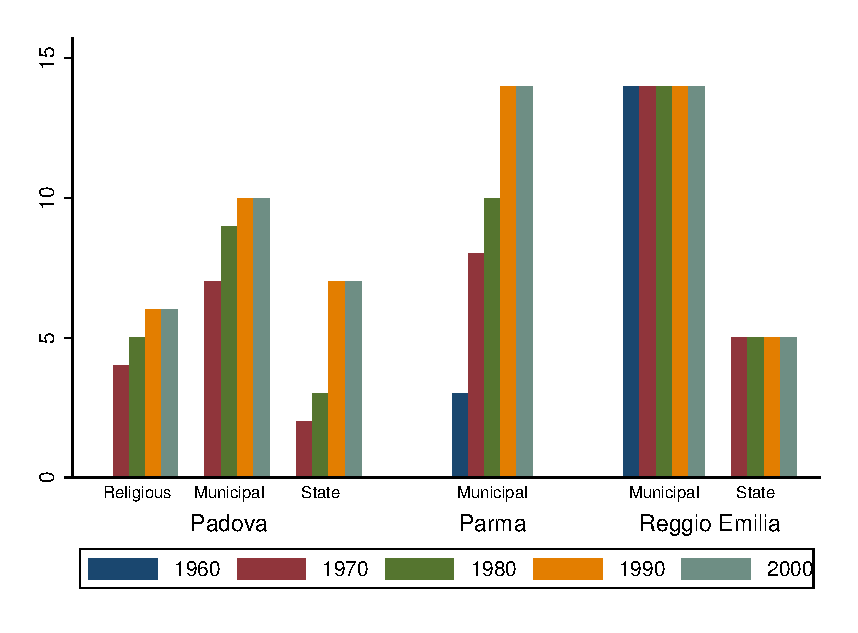
\includegraphics[width=\textwidth]{../../output/aggregateAdministrative.eps}
\end{subfigure}%
~
\begin{subfigure}[b]{0.55\textwidth}
	\caption{Number of Pedagogical Characteristics in Common with the Reggio Approach}\label{fig:agg-ped}
	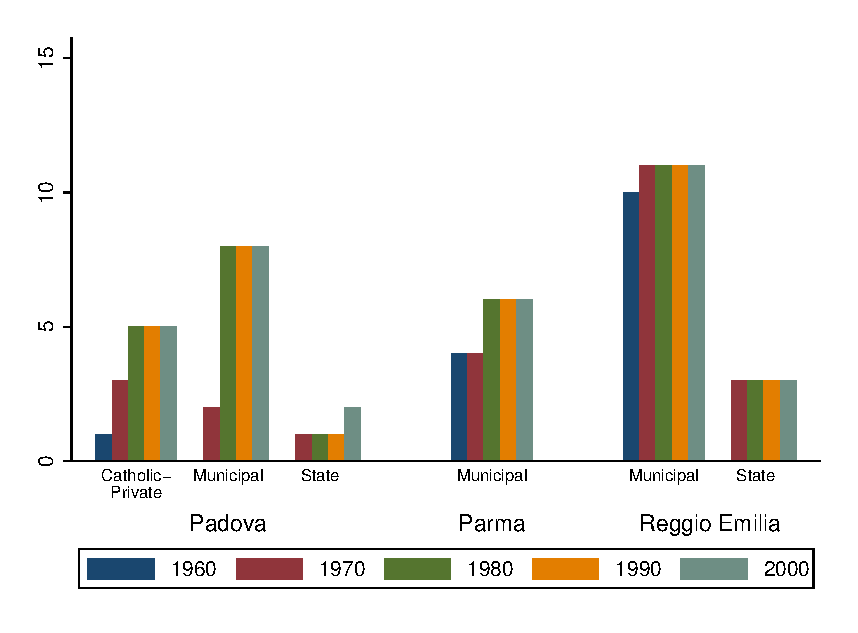
\includegraphics[width=\textwidth]{../../output/aggregatePedagogical.eps}
\end{subfigure}%
\end{center}
\raggedright \footnotesize Note: These graphs show the number of administrative and pedagogical components that each program has in common with the Reggio Approach. We consider 14 administrative components and 12 pedagogical components. One of the pedagogical components, following a set curriculum, was not present in the Reggio Approach. 
\end{figure}

% more details on survey results
The hours of center-based care is one commonality largely shared by the surveyed programs. All the programs except the state system in Padova offered additional hours for working families. Similarly, by the 1990s, all the surveyed systems received public funding. Some differences are seen in the teacher responsibilities. In the Reggio Approach, teachers have dedicated work hours to (i) engage with families, (ii) complete documentation tracking children's progress, and (iii) partake in professional development. These activities are not explicitly scheduled for teachers in Reggio Emilia and Padova's state schools. Time for professional development is similarly not scheduled for teachers in Padova's religious schools. Teachers in all surveyed systems, except the state schools, partook in documentation until the 1990ss even if it was not explicitly scheduled. After the 1990s, the state schools of Padova adopted this practice of documentation.

Municipal schools in the three cities shared priorities of enrolling economically disadvantaged children, children from a single-parent household, and children with disabilities. State schools in Reggio Emilia gave priority to economically disadvantaged children and those with disabilities, but not to those from a single-parent household. Religious schools in Padova did not prioritize enrollment of children from any of these groups indicating that the population of students in Padova's religious schools might have had more resources at home. % discuss if this is seen in the results

Some administrative aspects seen in the Reggio Approach were not widely implemented in other school systems as the aspects discussed above. These include the presence of a full-time educative coordinator and the inclusion of the non-classroom staff (e.g. kitchen and janitorial staff) in professional development trainings. It was not until the 1980s that at least one other system had a full-time educative coordinator. Even if the educative coordinator was part-time, as was the case for Padova's religious schools since the 1970s, the schedule of meeting biweekly with classroom staff remained. Parma municipal and more recently Padova municipal are the only other systems surveyed that include non-classroom staff in trainings.

When considering the pedagogical components in the survey, we also include components that were not present in the Reggio Approach in order to help contrast it with the other programs. These include (i) no religious education, including education that has moral subtext; (ii) no preset curriculum; and (iii) little influence of Montessori relative to the influence of Malaguzzi. 

Other schools, including municipal and state schools, included teaching with religious and moral themes, although less so for Parma and Padova's municipal schools after the 1970s. Instead of preset curriculum, the Reggio Approach includes project-based learning in which the projects are dictated by the children's interests and guided by the educative staff. Although the other municipal systems use curricula, they have included this project-based learning starting in the 1980s and 1990s. Finally, Montessori's teachings influenced Reggio Emilia's state schools and Padova's religious schools since the 1970s. Only more recently in the 200s do Padova's religious schools report being influenced by Malaguzzi's teachings. 

The structure of the classroom is similar between Reggio Emilia's municipal and state programs. In both cases, the classrooms have homogenous age groups and two co-teachers per class. Municipal schools in Parma and Padova included the same teacher structure starting in the 1980s. The set-up of the environment, both including natural light and objects and having a dedicated space for individual and small-group projects, are also seen in Parma and Padova's municipal systems.

There are two components of the Reggio Approach that were not as widely seen in the other systems. The first is the presence of an arts specialist. This has only been in seen as well in Padova's municipal school since the 1980s. It is important to note, however, that visual arts were used in a preschool setting in all the other programs by the 1980s.  

In addition to this historical context, we expand on shortcomings in the data that make more precise analysis difficult. It is clear that selection into the Reggio Approach is an important factor to consider. We presented estimates with different control sets to better understand the importance of observed background characteristics that can determine this selection. Controlling for more background characteristics, especially in the younger cohorts, makes the treatment effects more positive. With more precise background variables, such as a more complete variable for family income, we could better capture the disadvantage in the sample, allowing our estimates to be less biased. More background variables for the older cohorts would be especially useful considering there were fewer available for them.

%In Appendix~\ref{appendix:mlogit} we present the results from the multinomial logit model, which gives the marginal effect that a background characteristic has on attending a certain type of preschool arrangement.

Other variables would allow other analysis that attempts to account for differential selection on background characteristics. Although we attempted to construct instruments for enrollment, including distance to the nearest school and the presence of a grandparent nearby, these variables proved to be poor instruments, and not available for the older cohorts. Variables capturing the selection apart from background characteristics, such as complete tuition costs, would provide the opportunity to implement another specification to compute the treatment effects.

%\begin{itemize}
%	\item Discuss differences in eligibility requirements between cities and schools and how that might have contributed to differential selection
%	\item Data issues
%\end{itemize}




\clearpage

\bibliography{heckman}
\bibliographystyle{chicago}


\end{document}
